% study_notes.tex
\documentclass{article}
\usepackage[utf8]{inputenc}
\usepackage{amsmath}
\usepackage{graphicx}
\usepackage{hyperref}
\usepackage{geometry}
\usepackage{cite}
% Basic packages
\usepackage[utf8]{inputenc}
\usepackage[T1]{fontenc}
\usepackage[english]{babel}
\usepackage{lmodern}

\usepackage{color}
\usepackage{graphicx}
\usepackage{subcaption}

\usepackage{float}
\usepackage{cleveref}


\geometry{a4paper, margin=1in}

\title{Study Notes for AWR Tutorial}
\author{Your Name}
\date{\today}

\begin{document}

\maketitle

\begin{abstract}
These are study notes for the Advanced Writing and Research (AWR) tutorial.
\end{abstract}

\tableofcontents

\section{Introduction}
This is an introductory tutorial to use AWR from the Roland device.

\section{Videos}

\subsection{Design Troubleshooting for Stability Part 1}
Instability arises from the use of feedback and gain together. This can be controlled by adding loss or adjusting bypassing in the lab to stabilize the circuit.

\textbf{From AWR DE Tutorial 5}
\begin{itemize}
    \item After selecting the new schematic, name it and then press \texttt{Ctrl + L} to add elements.
    \item To see the details of a component, right-click and select \texttt{Help}.\cite{paper_2}
    \item You can add equations as in QUCS and use the factors in the component details.
    \item To tune an item or a factor on the graph, click the \texttt{Tune} tool above and then click on the factor; it will change to a blue color.
    \item Set the limit of the chosen factor and then click the tuner. It is behind the identifier tool that chose the factor to tune. You will see the variable tuner has limits and then you can change it above and below.
    \item To plot the output voltage (\( V_{out} \)), you need a voltmeter. Connect it in shunt with the load resistor \( R \) chosen from the element menu.
    \item To measure the DC characteristics of the amplifier (\( V_{out} \) vs \( V_{in} \)), you need a linear graph. Add a new measurement, select \texttt{Nonlinear} and then \texttt{Voltage}. Choose \( V_{DC} \) on the measurement component and place the voltmeter on the vertical axis. For the x-axis, use the voltage from the source.
    \item Click \texttt{Apply} and then choose the simulation tool on the schematic.
\end{itemize}

\textbf{From AWR DE Tutorial 6}
\begin{itemize}
    \item From the elements menu, you can also find the voltage source (V source). If it is AC, to measure it you will need a voltmeter similar to the one used on the load resistor.
    \item The working frequency is a global value defined for the overall project from the project options menu. Define the frequency range and then from the global units icon above, choose the frequency and change its unit to kHz in this case.
    \item The netlist file that can be imported into AWR has the extension \texttt{.cir}. From the netlist menu, select \texttt{Netlists} and then choose \texttt{Import Netlist}.
    \item With \texttt{Ctrl + K}, you can add the important netlist.
    \item After adding the symbols, you can change them from square and normal device shapes from \texttt{Properties > Symbols}, then choose the needed shape.
    \item To add the voltage source, add \texttt{DCVS} and \texttt{ACVS} from the elements.
\end{itemize}

\textbf{From AWR DE Tutorial 7}
\begin{itemize}
    \item The models that can be used in AWR are the PSpice models with \texttt{.cir} extension.
    \item These are called AWR netlist files.
    \item From \texttt{Steer 03.Wideband Amplifier Design Using the Negative Image Model, Part F}, we can see that the model used with the transistor is added in the data files above the graphs.
\end{itemize}

\textbf{From Impedance Matching AWR}
\begin{itemize}
    \item From project options, you can change many of the item units.
    \item You can use the cookbook for ADS and check the LNA simulation part and try to replicate it in AWR.
    \item To measure the input impedance, it is a linear measure, and you can find it on the graph after adding a new measure. Choose \( Z_{in} \).
    \item Define \( Z_{in} \) unit, the port number, and the source name. If there is a transmission line after the input port, it will appear.
    \item It is important to sweep the frequency and define the number of points for measurement to determine at which frequencies the device should read a measurement. This can be done from the project options window.
    \item To add another plot on the graph, click \texttt{Duplicate Measurement} and then from the window called \texttt{Modify Measurement}, you can add the changes between the two lines.
    \item For the 50-ohm resistor, if you change the \( Z_{in} \) measure from 75 ohms with the transmission line to 50 ohms, you will see matching at 50 ohms for \( Z_{in} \) real and the imaginary value is zero, indicating matching.
    \item In the case of 75 ohms with a 50-ohm transmission line, you will see the imaginary part increase with frequency from -20 to +20. If the imaginary part is greater than 0, it means positive reactance, indicating inductance, and negative reactance means it is capacitive.
    \item If you remove the resistor and use just the transmission line and simulate, you will see the real and imaginary parts are 0 ohms at 2.4 GHz if the transmission line is open, not grounded. If grounded, there will be a very large \( Z_{in} \) at 2.4 GHz.
    \item In the matching case, measure the impedance on the Smith chart and check where the point is for your frequency. Connect a series capacitor and a parallel inductor if the point on the Smith chart is on the capacitive part under the middle line. Then tune the values of C and L and check which one has a larger effect on the point. Tune it to get the point above on the inductive part, then with the capacitor value change it to reach the middle line indicating the point is totally matched.
    \item After adding a microstrip line with T-line used as a load, it should be matched when the length and the width give a 50-ohm for the material used on the substrate. In this case, the microstrip line and the T-line are 50-ohm, meaning they should be matched around the frequency of the T-line, which is 2.4 GHz. Matching can be seen from the impedance linear graph or from the Smith chart.
    \item If you have just one port, you will measure on Smith just \( S_{11} \). When measuring, it is a must to use the MSUB on the schematic to define the substrate for the transmission line. The values of the variables on the MSUB are taken from the window where we define the width and the length on the MSline, meaning \( \epsilon_r \) and tan \( \delta \) and so on.
    \item When matching with MSline, define the length and then you can add a parallel one in front of the MSline and define the length and tune it to get the matched point. Adding the admittance might help on Smith to get a line to move with it. On the new line, you can play with the width and the length.
    \item The microstrip TEE or MTEE is used to connect the MS lines instead of connecting them together, which might lead to parasitic capacitance. So the idea is to make the design and see the Smith chart and match with the MS lines, and then control the length and width of the MS lines to get the matched point. Then connect them with the MTEE with a dollar sign which will connect the three sides with the equivalent width for the line.
    \item If an MS line is not grounded, you need to connect the Mopen line, which is an MS line with open termination.
    \item To see the length of the MS lines, you can see the layout graph and then import the other component models that define the layout. AWR requires some experience because it does not always have the best documentation.
\end{itemize}

\textbf{Microstrip Antenna AWR Lab Video}
\begin{itemize} 
    \item This video is important for working with T-lines.
\end{itemize}

\section{Technical Note from the CEL Blog}
The CE3512K2 is an air cavity package structure which is effective in reducing RF power loss consumed by the packaging material. For HEMT, the gate has high impedance at DC, so there is only a need for bias at the drain and connecting \( V_g \) directly. The bias at the drain is sufficient to use just the inductor, and it should be high enough to provide good RF isolation at the operating frequency. The inductor can also be part of the matching network. A shunt capacitor provides a low impedance point, creating a low pass filter for noise and unwanted signals from the DC source. As frequency increases, parasitic effects become dominant, necessitating transmission line-based components in both bias and matching circuits.

\textbf{Transmission Line Matching}
The quarter wavelength (\( \lambda /4 \)) transmission line is a crucial element in RF design.
the (\(\lambda/4 \)) can replace he inductor on rf isolation. and for this technique there is no frequency limit.
Radial and rectangle open stub are the most common Tlines on rf.
thr coupling capacitors has to undesirable effects it has high insertion loss as a fraction of dB directly degrades the
noise figure by the same amount and the matching network is become complicated due to the parasitic effect of the high 
frequency capacitors.

output series capacitor has negatable impact on the circuit performance 

you will need bias tee if you you wanna exclude using the input capacitors to prevent dc coupling with the instrument during the measurement.
this only on noise figure measurement. 

Tlines component on the matching network usually used on the cas for the freq higher than  10Ghz

Ampleon is a good company for rf transistor with application note and references.
as stated on the website  edaboard.com   after you have the transistor model you can chose a bias point then stability analysis 
with Rollet factor then design the input and output matching. also the power transistor has optimum load impedance
that maximize the delivered power or the gain.

one simple measurement is to make representation for the S param and then compare between QUCS and AWR 


 \textbf for Simulation 

 add S2p on the data files by import then add it on the schematic as rectangle then click and from Properties change the symbol.
 then follow the circuit stubs as on the Matching with the AWR video.
 the bias circuit is to design the bias point and the matching to work on  50ohm 
 on HEMT  transistor has highrt breakdown voltage and high operational temp.
$
\Gamma (S) = \Gamma (opt) $  must be first for LNA
connect the bias circuit and define the bias voltaged and calculate Rg and Rd and the capacitor and the inductors






\section{From github (https://github.com/aliruveycan/Maximum-Earnings-using-AWR-Microwave-Office-Amplifier-Design-and-Simulation.git)}

to simulate the  transistor on the data files upload the s parameter file 
and on the graphs plot all S parameters graphs.

then you can match with the Tlines  length as on the AWR 1 hour tutorial for Matching.








\section{Diffrent pdf notes from google Image}
\textbf{From Ultra wid band amp by chengcheng Xu}
Rf amplifier is used to amplify small signal amplitude to a large amplitude  in transmission and receive signal from antennas.


if the BW from 1.5 to 3.5  Ghz it means that  the amplifier can  be called 2 GHz amp so our amplifer can be called 
1GHz  or 800 MHz  or 600MHz   amplifer for the SNSPDs 


 Not understood   phrase is the final gain is 20 dB with the power gain slightly below 30 dBm.

 if the transistor IV curve is mostly linear then the output signal gain will be linear otherwise gain will be non linear.

 Class A amplifier has poor efficiency when converting the dc power to high freq output power 
 the lost power will br converted to heat on the device this power that is not converted to rf power 
but it provide great output to input linearity 
#

Class B more efficient than A but it scarifies the output linearity to  input signal ratio. lead to distortion on the output
signal half of the signal only amplified 

push pull configuration with two transistor may solve the class B amplifier issue.

if the spice model is not provided so the setup a bias network is not important you will use on the s2p file form the 
provider then you need to match the output of the transistor to the output matching circuit 
also consider the stability of the amplifier if it is conditional on unconditional stable.

the S22 matching with the output matching network is created first than the inpupt matching network 

if S11 is not matched all the input power will not be deliver to the amplifier 

the biasing circuit or bias point use one that is recommended from the the provider bias points means the points for the 
s2p files that provided Vds and Vgs and Id  

chose the bias point that has gain near to your interested freq on the thesis they use s2p at 3v 60 mA bias this can be show from the graph for 
MSG/MAG and S21 dB  you see that S21 has gain at the needed frequency.


this bias point also avilable on the AWR software so no need to import the file on the Microwave office software 


P1dB  compression point is also important  as the transistor it self is not linear so the output / input ratio can't be linear
 
it is defined as the point where the device output power and the linear model output different
by 1dB.

this point where the device also start to provide Nonlinear behavior so you look at the p1dB point on the data sheet 

if you wanna use another transistor you should follow the same process.

the FPD2250 has 1dB point 31dBm  and if the gain is 10dB  so the max power input to the transistor
is 21dBm so you need to see the conversion of the power values to dBm and check the P1dB effect. the 21dBm will be 
above the output of the 1 st stage.

the stability is not related to which gain value of BW is the device it self is unstable  this will not has an effect
on what gain or other parameter so we need to use stable network to prevent oscillating output


the stability on Microwave office is tested by K() and B1 parameter and also by SCIR1() and SCIR2() parameters of the device

K>1 and B not < 0 

SCRR 1 will create solid line  and dashed lines circles the inside or out side the l´solid line circle 

the  solid circle will be the stable one. the goal is to be inside the stable region 

\textbf{ Design steps}
\begin{itemize}
    \item add the transistor model and change it to symbol or leave it as it is.
    \item check also if it is avilable on AWR or not at the beaning
    \item design a bias point circuit should be stable or should be called stability circuit. ther is no voltage sources as on fig on the tutorial just Rd and Rout and Rg and the two ports also you  might need to use MSline and control it's length tune the component then see the stability for K and B values.
    \item the above  step is  reoeated for the two the stages on thier own.
    \item this stability test can be done on smith plot with the circles need te studied alone.
\end{itemize}

\textbf{Wideband Matching}
\begin{itemize}
    \item the goal is to has a Wideband at the first gain is not important at this point as the BW.
    \item so Gmax is not needed now check table one on the tutorial pdf
    \item matching method are Chebyshev matching  and lumped elements matching
    \item Chebyshev matching is based on Chebyshev polynomial and the matching network is mostly consist of quarter wave transformer
    and from the BW and quarter wave transformer section number the impedance of each quarter wave transistor is generated
    Chebyshev Matching is on figure 12
    \item  then you need to see the matching on smith see S11 and S22 it should be nearly perfect match 
    means it is circulated around the center point smith plot.
    \item  as shown on figure 12 Chebyshev has 6 Tline for each S11 and S22 and the and the length of the quarter wave transistor
    need to be quarter of the signal wavelength. so the reault now for Rf application is not realestic and the
    and the design will be very large and amplifier detentions will be large
    \item so the Chebyshev matching is not implemented  here.
\end{itemize}





\textbf{lumped element match}
\begin{itemize}
    \item 
\end{itemize}




\section{matching}

on smith for any point to match it move with circle until you get a point on a circle that pass by the smith center 
which is 50 ohm matched.

on impedance smith series R go go right toward the center line 
series C goes down
series L goes up


on the admittance plane the shunt R,L,C  goes the same L up 
C down but R left.

\textbf{on Lec 7 impedance match with smith video is very nice}

if $$z_o = 50 ohm and Z_s = 50 ohm so Z_i the normalized impedance is 1 means full matched$$
$Z_i$ which is represented on smith chart 

adding resistor will add loss to your design so using L and C is is enough and better.
impedance match with the Tlines is very diffcult compared to Lumped element but the idea is the 
same there is numerating on smith for the matching lines.
bit the middle line for the real is the same but the imagnary numbers are written now interms of \Lambda.




\textbf{Txline  feature from AER Videos}

from tools chose txline it is used to know how much width should the line be to be $50 ohm$
or how length should be to 90 deg at 80 Ghz for example
on the txline window change to mm on length and width 
using the arrow on the middle to change between the calcuation then use the length and width on thes chematic then simulate to see 
the smith chart  you will see the point is on the middle if smitt


\textbf{Sweep feature}
on the parameter you want sweep click right then chose sweep  define a start and end and steps.
 and define also by equation a value to initialize the variable.
\textbf{Reflection coefficient measurement}
from the graph and S11 measure but at the beginning you have to add measure port at the input 
all of that is on the polar plot not smith
then tune the Tline length.
and see the effect on S11 

if you change the port to harmonic balance port you will be able to see the 
I V values on this device. time waveforms  of I V.
on elements it is called port1
you will see the wave source.after it you need a V meter or I meter 
from element chose V_meter and also I meter 
I meter on series after port and v meter on shunt.
from the graph rectangle then Nonlinear graphs then voltage then vtime.

on plot chose properties then measurement then  chose which graph on left and which on right. side.

on the Tline is length 0  the I V time relation are on phase when change the length the VSWR is the same and the 
real part of the reflection coefficient is the same  but hte phase deg changes always
this means the phase difference between IVtime relation will change.

due to the phase changes the Tline is considered as network from inductors series and capacitor parallel
with the the voltage source.

VSWr is the ration between $$V_max$$ / $$V_min$$





\textbf{there are some simulation AWR videos on the Microwave labcast channel}


\textbf{Simulation} 
\begin{itemize}
    
    \item import the sparmeter and make graph for the device at the beganing before anything.
    \item then you can make your graph from the graph tool
    \item first stabilize your circuit connet in out series R and shunt R at the out this will leads to uncoditional stability.
    \item then you can check that by the by K measure or SCIR1 ans SCIR2 for stability circle.
    \item now need to match over the wide band this is most important than getting gain. so BW is the important now
    \item the Match step is the most difficult this can be by the TLines and the lumped elements 
    \item most popular on AWR the Tline method from the Txline tool you can characterize your Tline properties.
    \item Match output before the input it is easy and important for the gain means match s22 of the transistor with the output load or matching.
    \item then Match the input S11 for the transistor with the input circuit to be sure that the power will be deceived to the transistor otherwise it will not.
    \item now Design  input match and output match sepertly and check them on smith the trick here is to make the whore freq range around the match point middle of smith
    \item and define only the operating or project frequencies on fron Dc to 1 ghz and define for th txline frequencies the middle point 500 MHz or less it means to make the Wideband match you need to match around the middle frequency.
    \item after you make the matching circuits make blocks and connect them to the in and out of the transistor 
    \item then check the gain now.
    \item then change the port to source nd simulate the power on the device to see the total power output on this case you will see only the part where the S parametr measured mean the linear region not the whole characterstcis this due to no Nonlinear model avilable for the transistor
    \item and due to no Nonlinear model the Nonlinearity  mean P1dB and OPI3 points of the device will be read only from the datasheet as mentioned on the pdf tutorial by chengcheng zu.
    on the Tlines from the txline which is considered to be real Tline insted of the ideal one.
    you will use the stability T junctions  when connect 3 Diffrent Txlines.
\end{itemize}

\textbf{Matching Circuit Notes}
\begin{itemize}
    \item \textbf{From AWR Matching Tutorial}
    \item An ideal transmission line (Tline) is lossless and provides a perfect phase delay at a specific frequency, similar to what was discussed in class.
    \item Under the transmission lines menu, you will find the phase menu, where you can choose `Tlin` and `Tloc` options. These are used for the lossless case.
    \item For the Tline, \(Z_0\) is the characteristic impedance. Keep it at $50\,\Omega$. EL is the electrical length, which is not the physical length, but the phase delay in degrees that will apply to the signal. \(F_0\) is the center frequency, which is crucial for determining EL.
    \item To simulate the input impedance in ohms from the linear curves, choose `Zin` and select only the magnitude. Then, generate your graph and measure from Port 1.
    \item The real part of Zin represents the resistance in ohms, while the imaginary part of Zin shows the reactance, which defines whether the circuit behaves capacitively or inductively (negative or positive reactance). This is where the matching process begins.
    \item If you measure the Zin for the Tline with only a ground connection, it will show a large value at the center frequency, indicating an open circuit due to the high impedance.
    \item If you want to control a frequency on the Smith chart, set it as the central frequency on the Tlines, observe its point on the Smith chart, and then move it up and down based on the admittance and impedance plots. Note that using resistors is not preferred, as they introduce losses.
    \item When starting to match with lumped elements, always begin with the L-network of an inductor (L) and a capacitor (C) together, then adjust it. Notice that increasing the capacitance lowers the impedance since \( Z = \frac{j}{\omega C} \).
    \item After matching on the Zin Smith charts with a complex magnitude, you can create an S11 graph and observe the value at the matched frequency in dB.
    \item The problem with ideal Tlines is that they are not practical; they don't account for losses, junction connections, or various parasitics.
    \item To work with real Tlines, you need a new schematic.
    \item Real Tlines rotate around the center point by a specific amount, unlike LC components.
    \item After defining the microstrip line (MSline) based on the Txline tool, prepare the substrate for your measurements using the same tool.
    \item To achieve matching, add series and parallel Tlines and adjust their length and width.
    \item Simulate a T-shaped Tline on the layout to check the design before fabrication. When connecting more than one Tline with a T-junction, ensure that the widths of the junction sides and the Tlines are consistent. Only change the length. The length should not exceed 20 mm to maintain the dimensions of the PCB after fabrication.
    \item The junction is called MTEE, and there is another variant called $MTEE\$$, which automatically adjusts the widths if you have different width Tlines.
    \item For the open-ended Tline, use `Mopen` to terminate the Tline.
    \item There is a tool called `Snap Together` on the toolbar. Just select all Tlines on the layout and press it, and everything will be connected automatically. The tool is located next to the `Tuner` tool.
    \item If you want to solve everything in a 3D simulation, you will need an EM simulation, which is quite difficult.
\end{itemize}


\textbf{from edaboard}
\begin{itemize}
    \item power transistor have optimum load impedance that maximize either the delivered power or the power gian 
    \item if you connect the the pspice model for thr transistor  you can use the IVVURVE tool to mesure the graph for the transistor.just connect the drain and the gate.
    \item also you could add the models for lumped elements like C or L and R  you need to import the model on the net files.
    \textbf{tips}
    \item you can add series R at the gate to get stable device the output match is enough to use the output capacitor and the bias Ld , Rd with capacitor or without.
    \item also the gate the bias with Lg and series and parrellel resistor.
    \item also the matching of the inpupt is the most important mostly done with LC circuits 
    \item as on the figure 2 sreies L and 2 parrellel C with the coupling capacitor. note the capacitors are infront the inductors.
    \item also the output match is done on the same way but  it arranged this way series L  parrellel C and then repeated one time.
    \item on smith you measure S11 and S11* 
    \item tuners helps alot to find the points on smith.
    \item search about LTuner tool that show smith chart as like boxing the the matching circuit. it is connect after the ports directly means the capacitor are inside it.#
    \item also omn this circuit the inductor and the reistor and are in series for the biasing.
    \item the port impedance musst be conjugate of the optimum load ot sourse impedence
    \item there are power matching and conjugate matching
\end{itemize}





\textbf{optimzation}
\begin{itemize}
    \item to begin optimization from  view menu chose variable browser then mark on optmize foor the varible you want.
    \item  also there constrain option to define min and max values no need for it now
    \item after you mark to optimize chose the optimzer goal from the project list 
    \item then chose the parametr you want control just S11 or S22  or any other measuremet 
    \item define the value at goal start option
    \item then define goal type > or < or = 
    \item then define the bandwifth you want get this value on it on min and max options 
    \item then you will find a mark on the graph you can move it on the graph and change the optimization goal  by mouse
    \item repeat the process with other curves then see the other marker on the graph for the other otimizer goal .
    \item then in simulate menu click optimize 
    \item on the menu chose Random local for the optimization method 
    \item Mac iteration means how many times the circuit simulated greater number better result but takes longer  

\end{itemize} 


\textbf{Dc biaing at the end}
\begin{itemize}
    \item when you chose a s parameter file it has a  Id and Vds values the bias Vdd is not Vds 
    \item do  use Rd which will give you the needed Id and use the Vdd to get the nedded Vds 
    \item using High Rg is nice to don't didturb the measurments for matching.
    \item use I meter and V meter to meaure these values.
    \item 
\end{itemize}


\textbf{From Microwave Labcast Lecture 9}

\textbf{From Microwave Labcast Lecture 9}

\begin{itemize}
    \item Oscillating occurs due to Amplifier + Feedback. Some slides from the video are shown in \cref{stability1,stability2}.
    
    \begin{figure}[H]
        \centering
        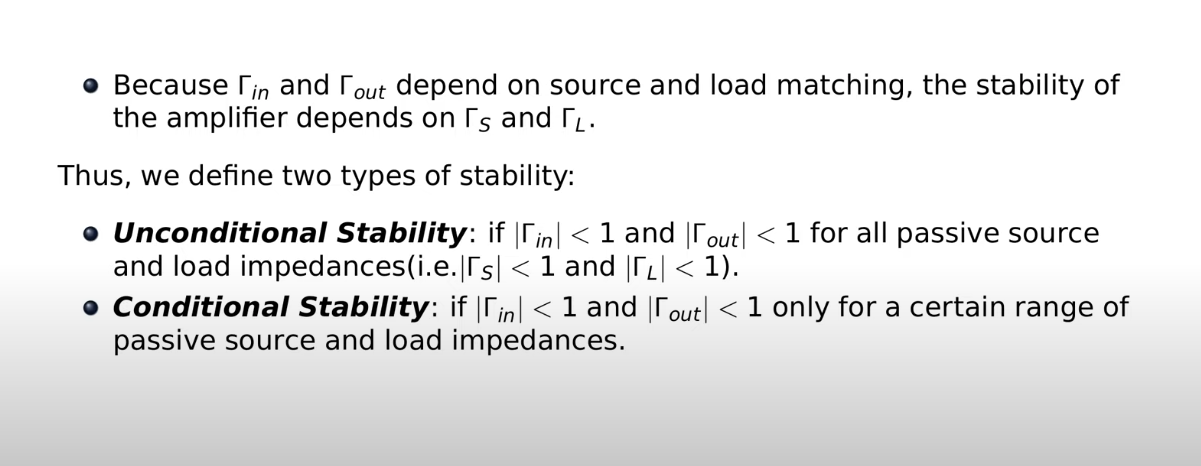
\includegraphics[width=0.8\textwidth]{figures/stability 1.png}
        \caption{Stability Figure 1}
        \label{stability1}
    \end{figure}

    \begin{figure}[H]
        \centering
        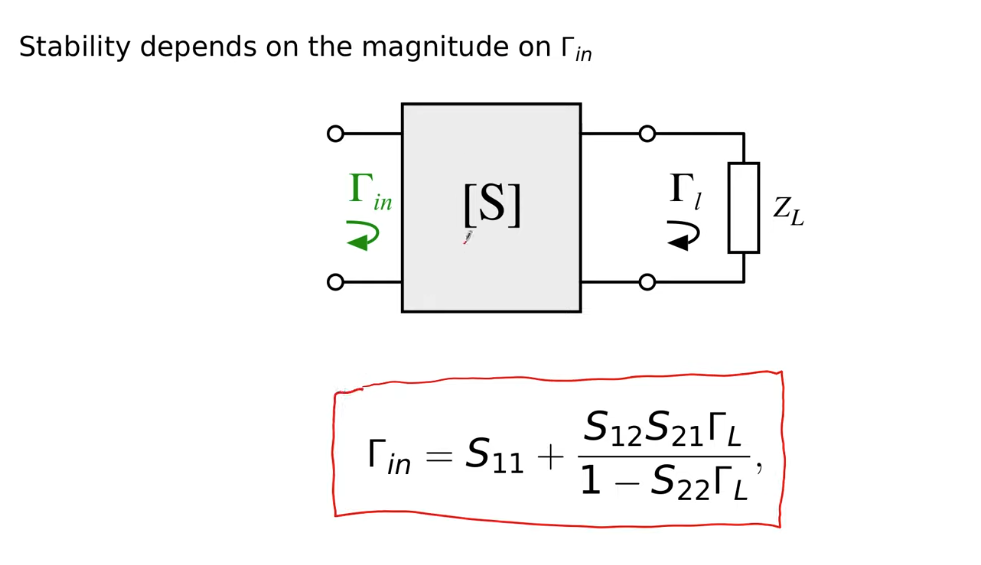
\includegraphics[width=0.8\textwidth]{figures/stability 2.png}
        \caption{Stability Figure 2}
        \label{stability2}
    \end{figure}

    
    \begin{figure}[H]
        \centering
        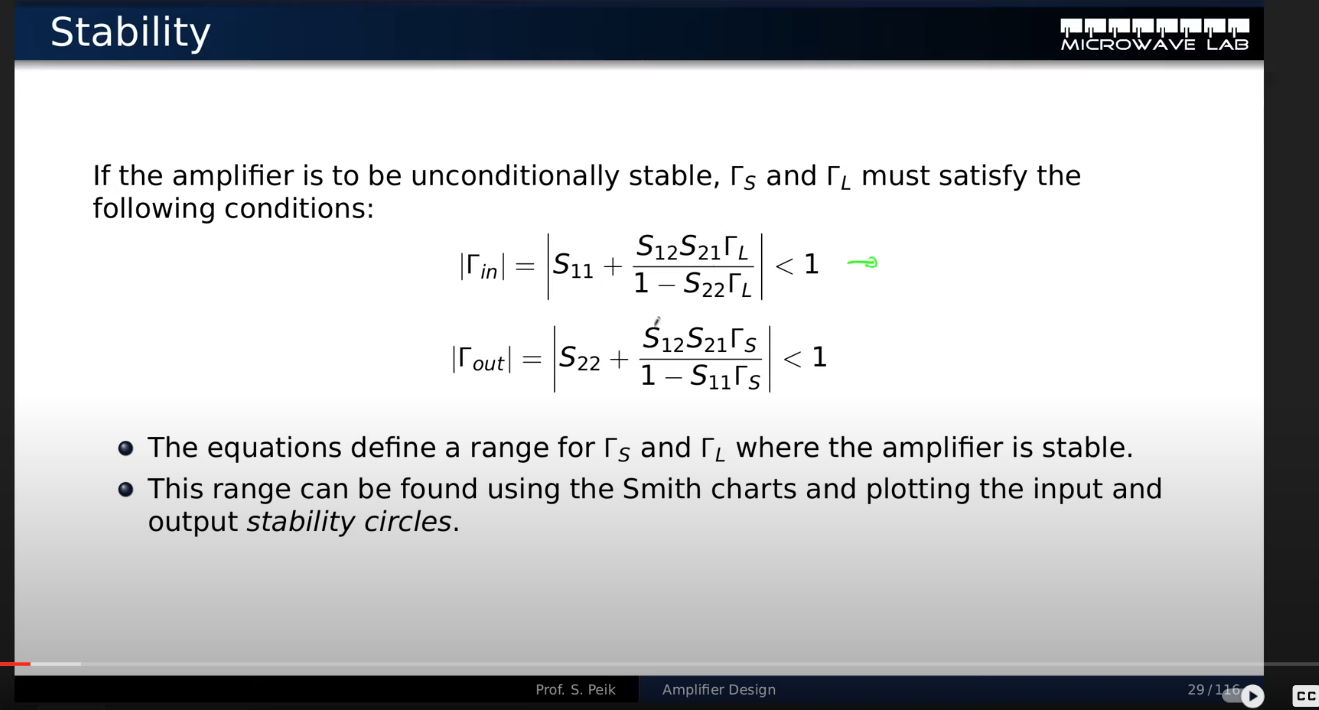
\includegraphics[width=0.8\textwidth]{figures/stability 3.png}
        \caption{Stability Figure 3}
        \label{stability3}
    \end{figure}

     
    \begin{figure}[H]
        \centering
        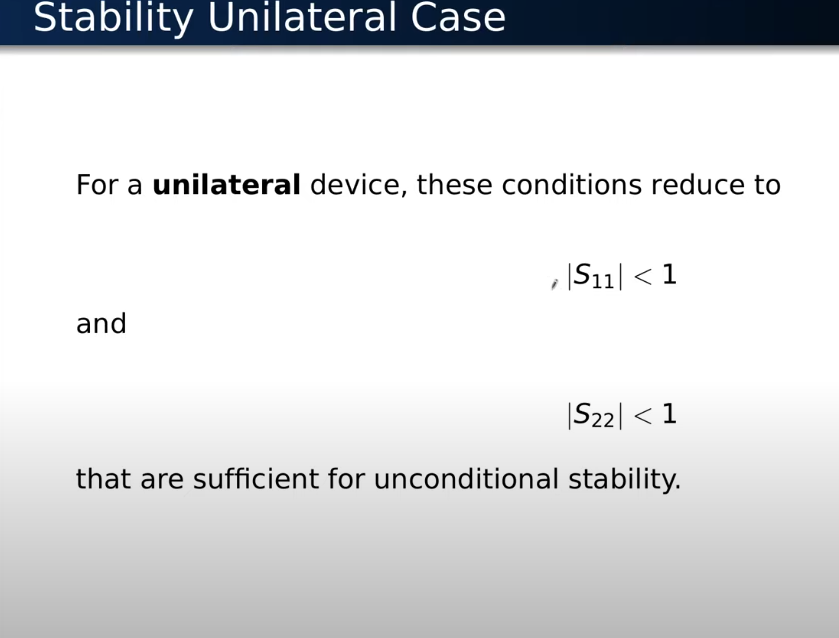
\includegraphics[width=0.8\textwidth]{figures/stability 4.png}
        \caption{Stabiliy for transistor and amplifier}
        \label{stability3}
    \end{figure}
    \item  after the derivation for the Gamma in aout you get this for the C and R  
    C is the center of complex numbers and R is the radius for the real numbers 
       
    \begin{figure}[H]
        \centering
        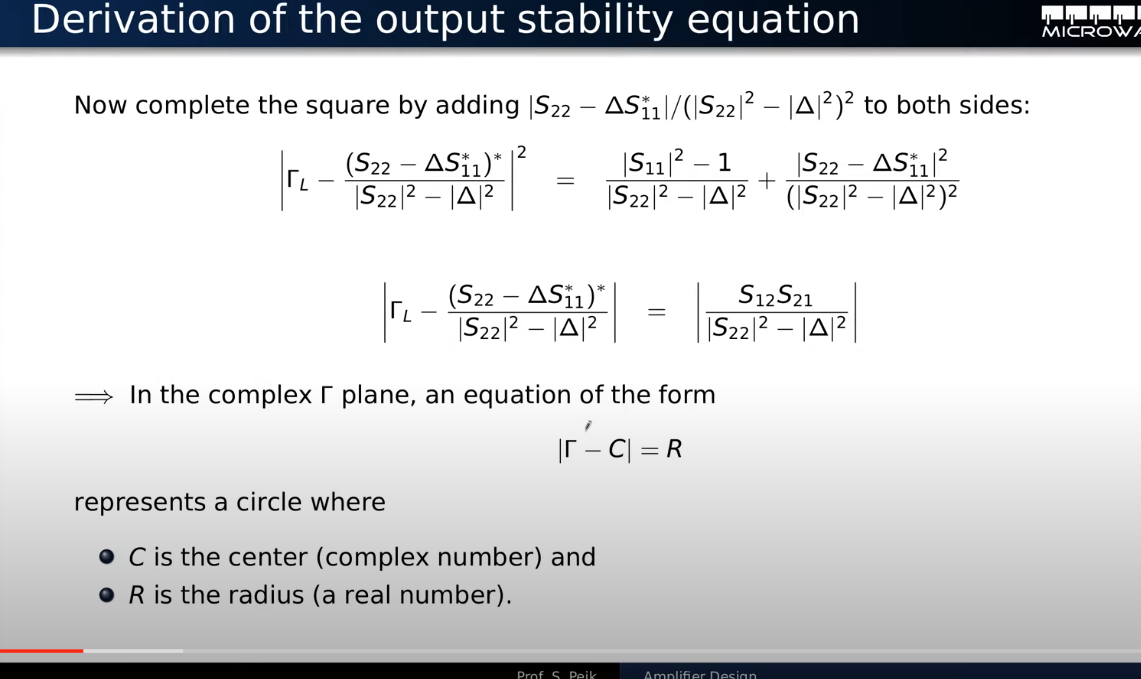
\includegraphics[width=0.8\textwidth]{figures/stability 5.png}
        \caption{Stabiliy for transistor and amplifier}
        \label{stability5}
    \end{figure}
    \begin{figure}[H]
        \centering
        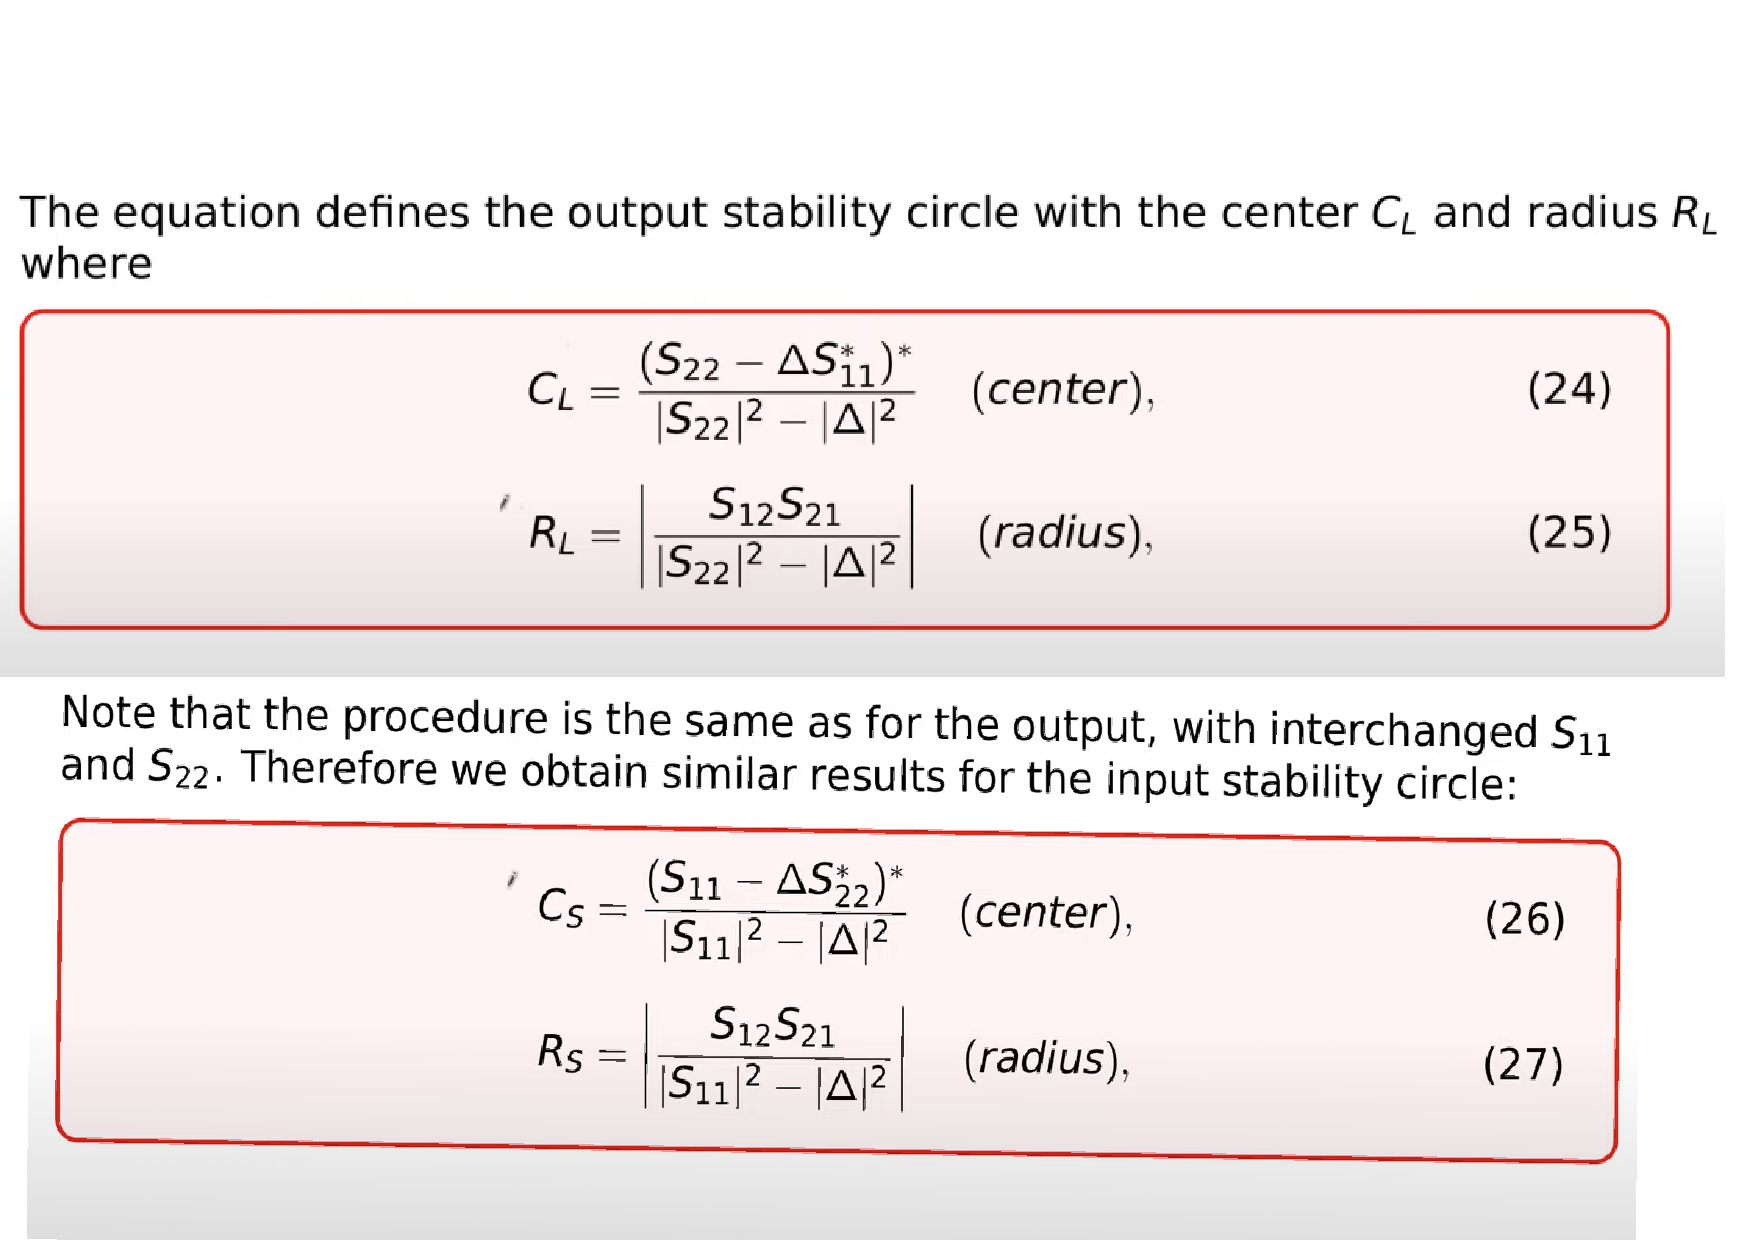
\includegraphics[width=0.8\textwidth]{figures/stability 5.pdf}
        \caption{Stabiliy for transistor and amplifier}
        \label{stability5}
    \end{figure}
   

    \begin{figure}[H]
        \centering
        \includegraphics[width=0.8\textwidth]{figures/stability 7.pdf}
        \caption{Stabiliy for transistor and amplifier}
        \label{stability5}
    \end{figure}


    \begin{figure}[H]
        \centering
        \includegraphics[width=0.8\textwidth]{figures/stability 8.pdf}
        \caption{Stabiliy for transistor and amplifier}
        \label{stability5}
    \end{figure}

    \begin{figure}[H]
        \centering
        \includegraphics[width=0.8\textwidth]{figures/stability 9.pdf}
        \caption{Stabiliy for transistor and amplifier}
        \label{stability5}
    \end{figure}

    \begin{figure}[H]
        \centering
        \includegraphics[width=0.8\textwidth]{figures/stability 10.pdf}
        \caption{Stabiliy for transistor and amplifier}
        \label{stability5}
    \end{figure}




\end{itemize}




\textbf{from sim videos}
\begin{itemize}
    \item this some pictures for some tricks used on the video during worrking with Tlines. as shown on fig \cref{simV1}
    \begin{figure}[H]
        \centering
        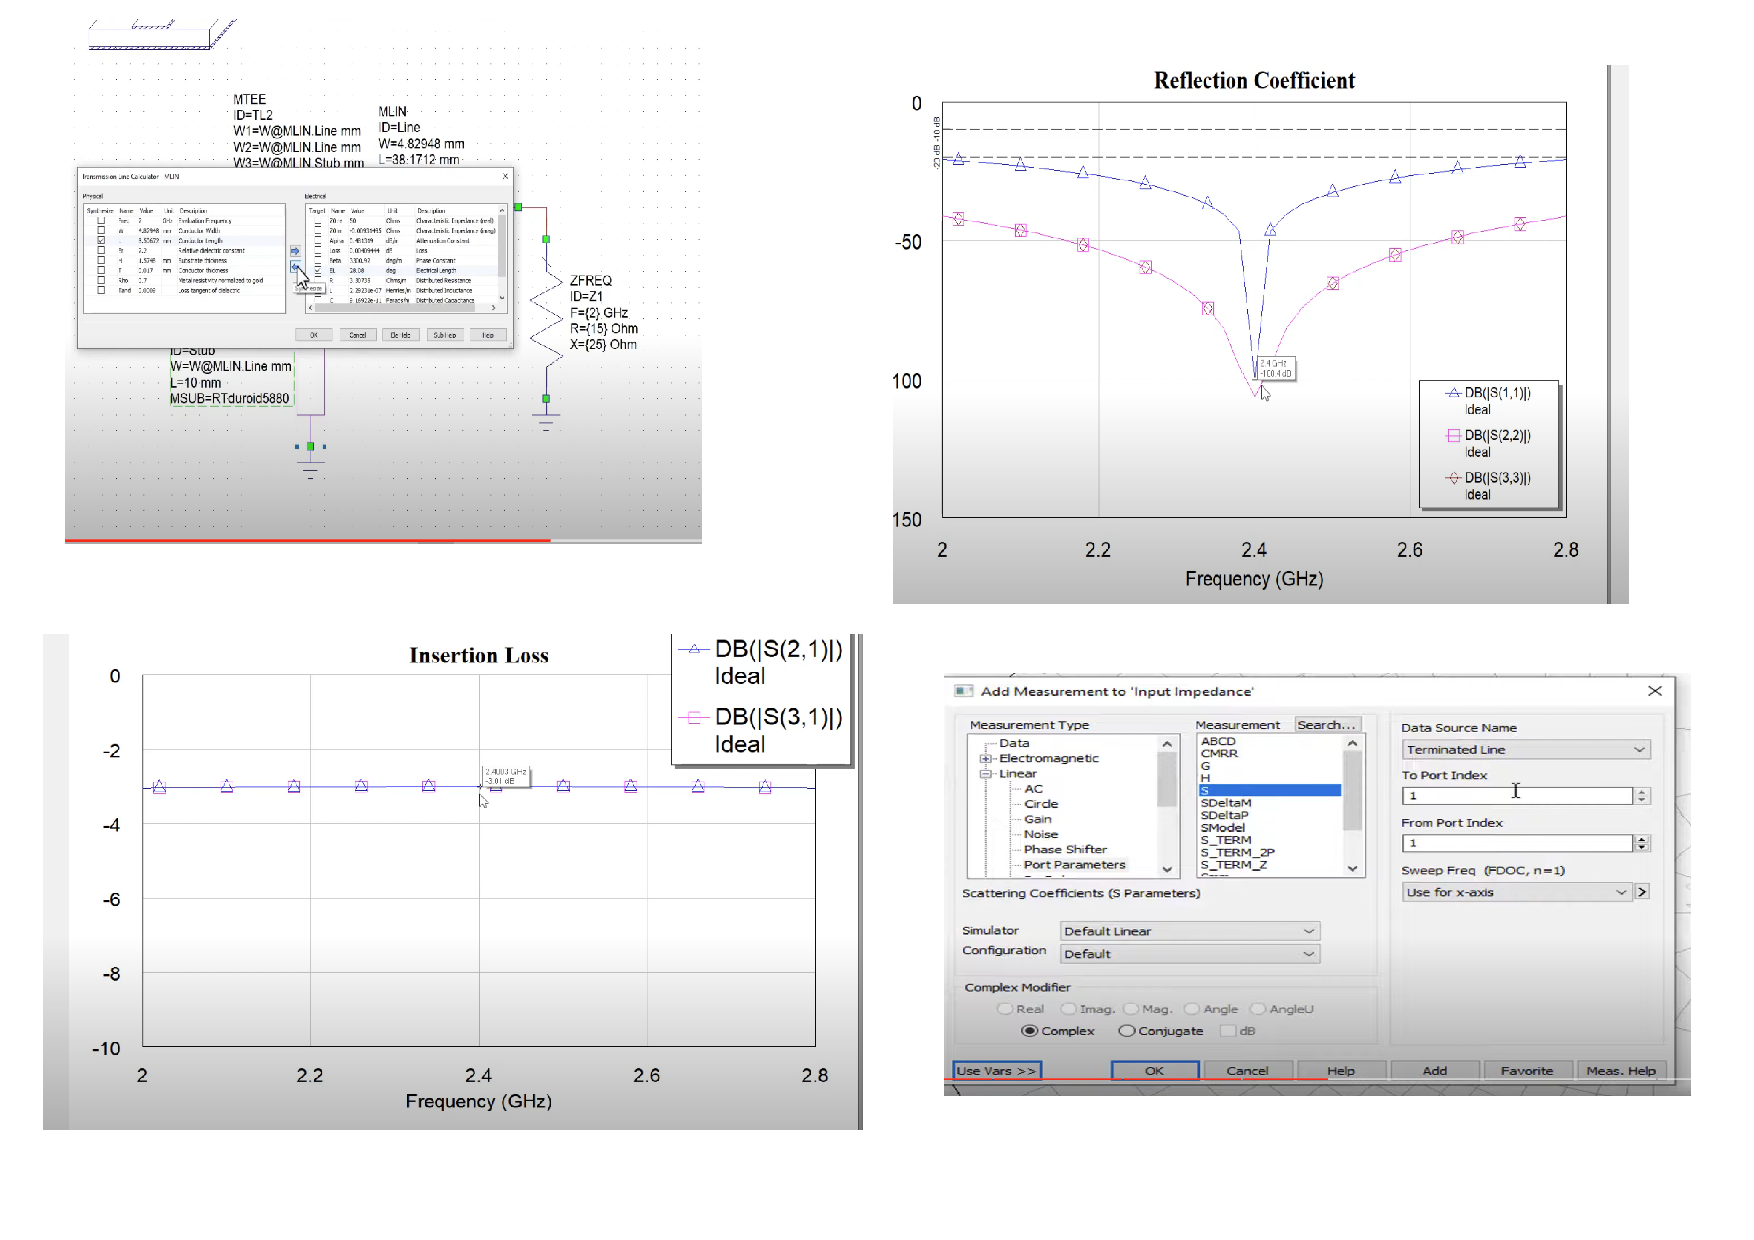
\includegraphics[width=0.8\textwidth]{figures/SimV1.pdf}
        \caption{some tricks to write the tlines width and length also to use the tline calculator and update the line automatically also how to meaure the indertion loss and the 
        the reflection coiffecnt and also the input impedance}
        \label{simV1}
    \end{figure}

\end{itemize}

\textbf{What to do to design}
\begin{itemize}
    \item stability ba K and delta  or SCIR_IJ(1,2) and SCIR_IJ(2,1) on smith to be sure that all circles outside the smith means unconditional stable.the k as on the pdf file on my laptop.
    
    stability wit the SCIR1 and SCIR2  for 22 and 11  should the spesified freq circle should be outside the the smith plot.
    all stability circles should be outside.
    the shunt resistor takes the circles outside to the open side right side of smith
    the series resistor takes the circles outside of smith from the left side  or the short circuit side.



    stability with  MU1 ans MU2  and chose port 22  for the two values for the output stability A
    also this repeated with thr inpupt match. don't chose a unit leave it normalised .
     MU > 1 for the stability with MU test.
     MU is the distance of the closed point of the stability circle to the center of the smith chart
     if MU < 1  the design will be potentialy Instability.


     stability with K>1 and delta <1 I think also the it works for 11 and 22 
     stabilize the design could reduce the gain also.


     for the stability test add to the transistor inpur and output capacitors and the L shocks inductor on the line for the biasing circuit.
     then amke the stability test
     define the s parameter simulatioon from the points for the freq range for the transistor 
     
     like this circuit on \cref{stability00}
     \begin{figure}[H]
        \centering
        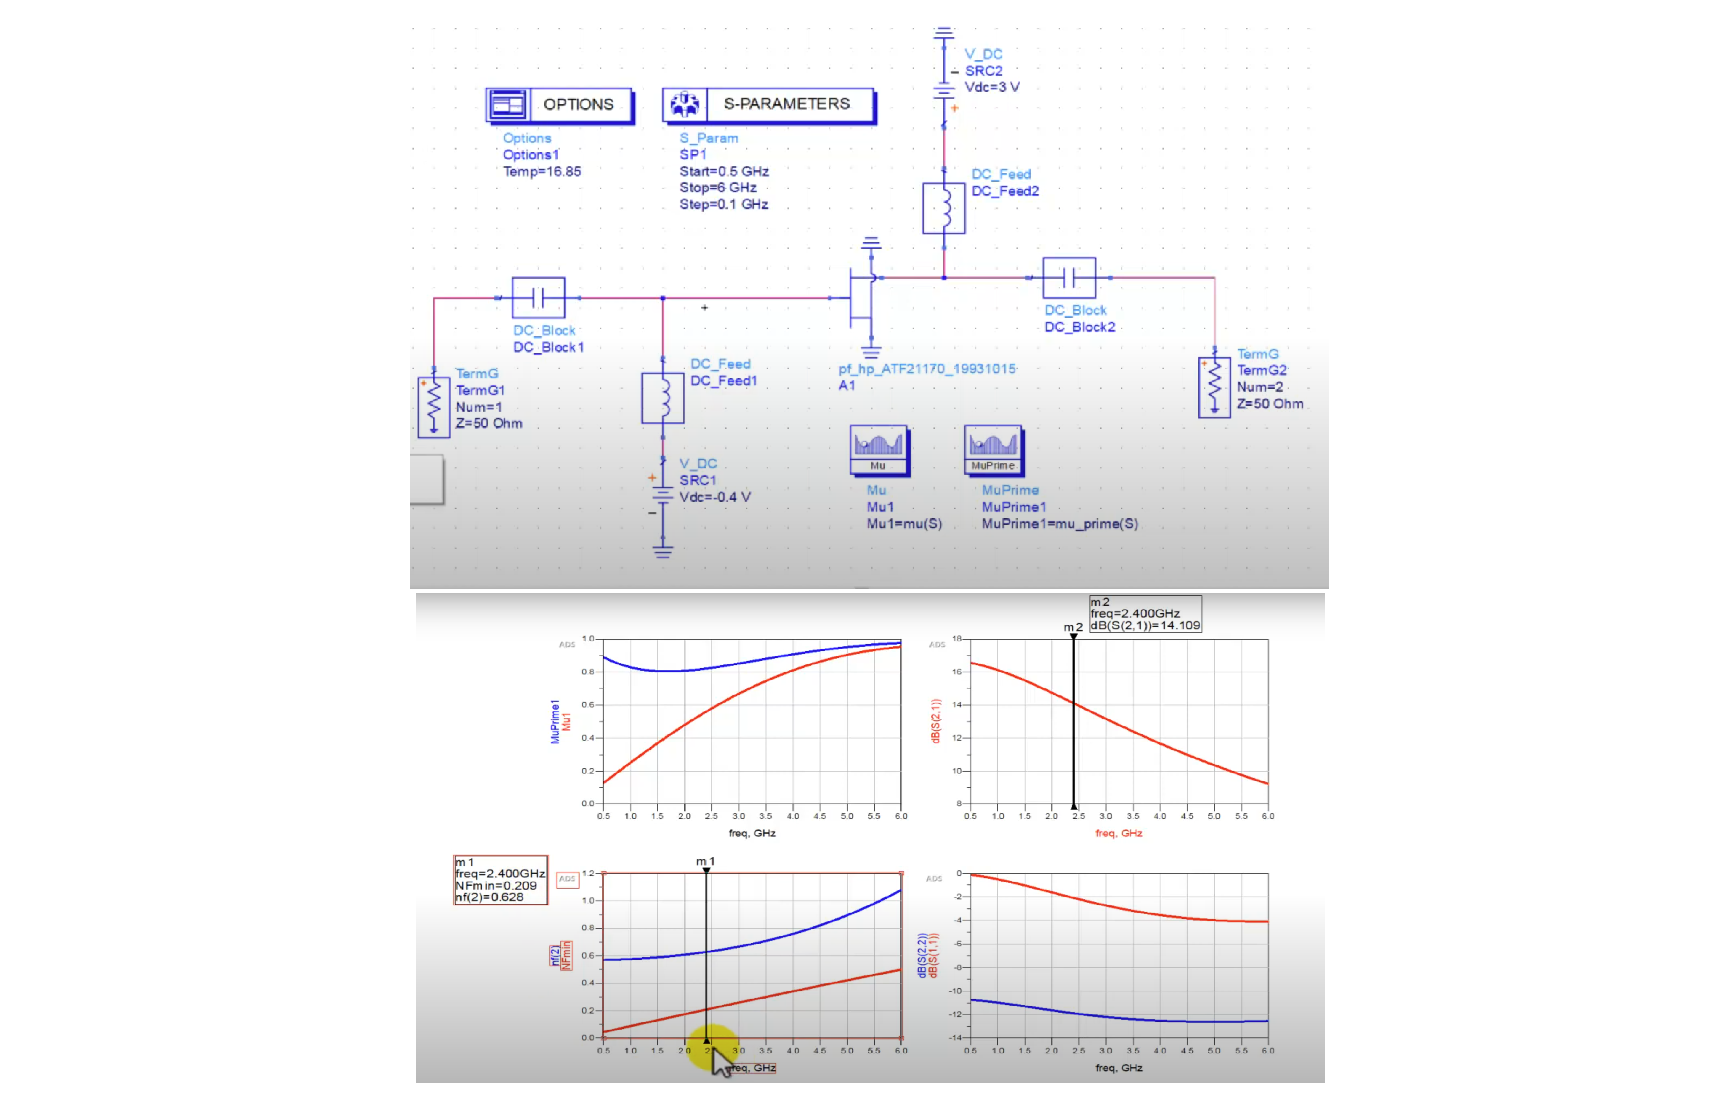
\includegraphics[width=0.8\textwidth]{figures/stability00.pdf}
        \caption{Stabiliy for transistor and amplifier}
        \label{stability00}
    \end{figure}
    \begin{figure}[H]
        \centering
        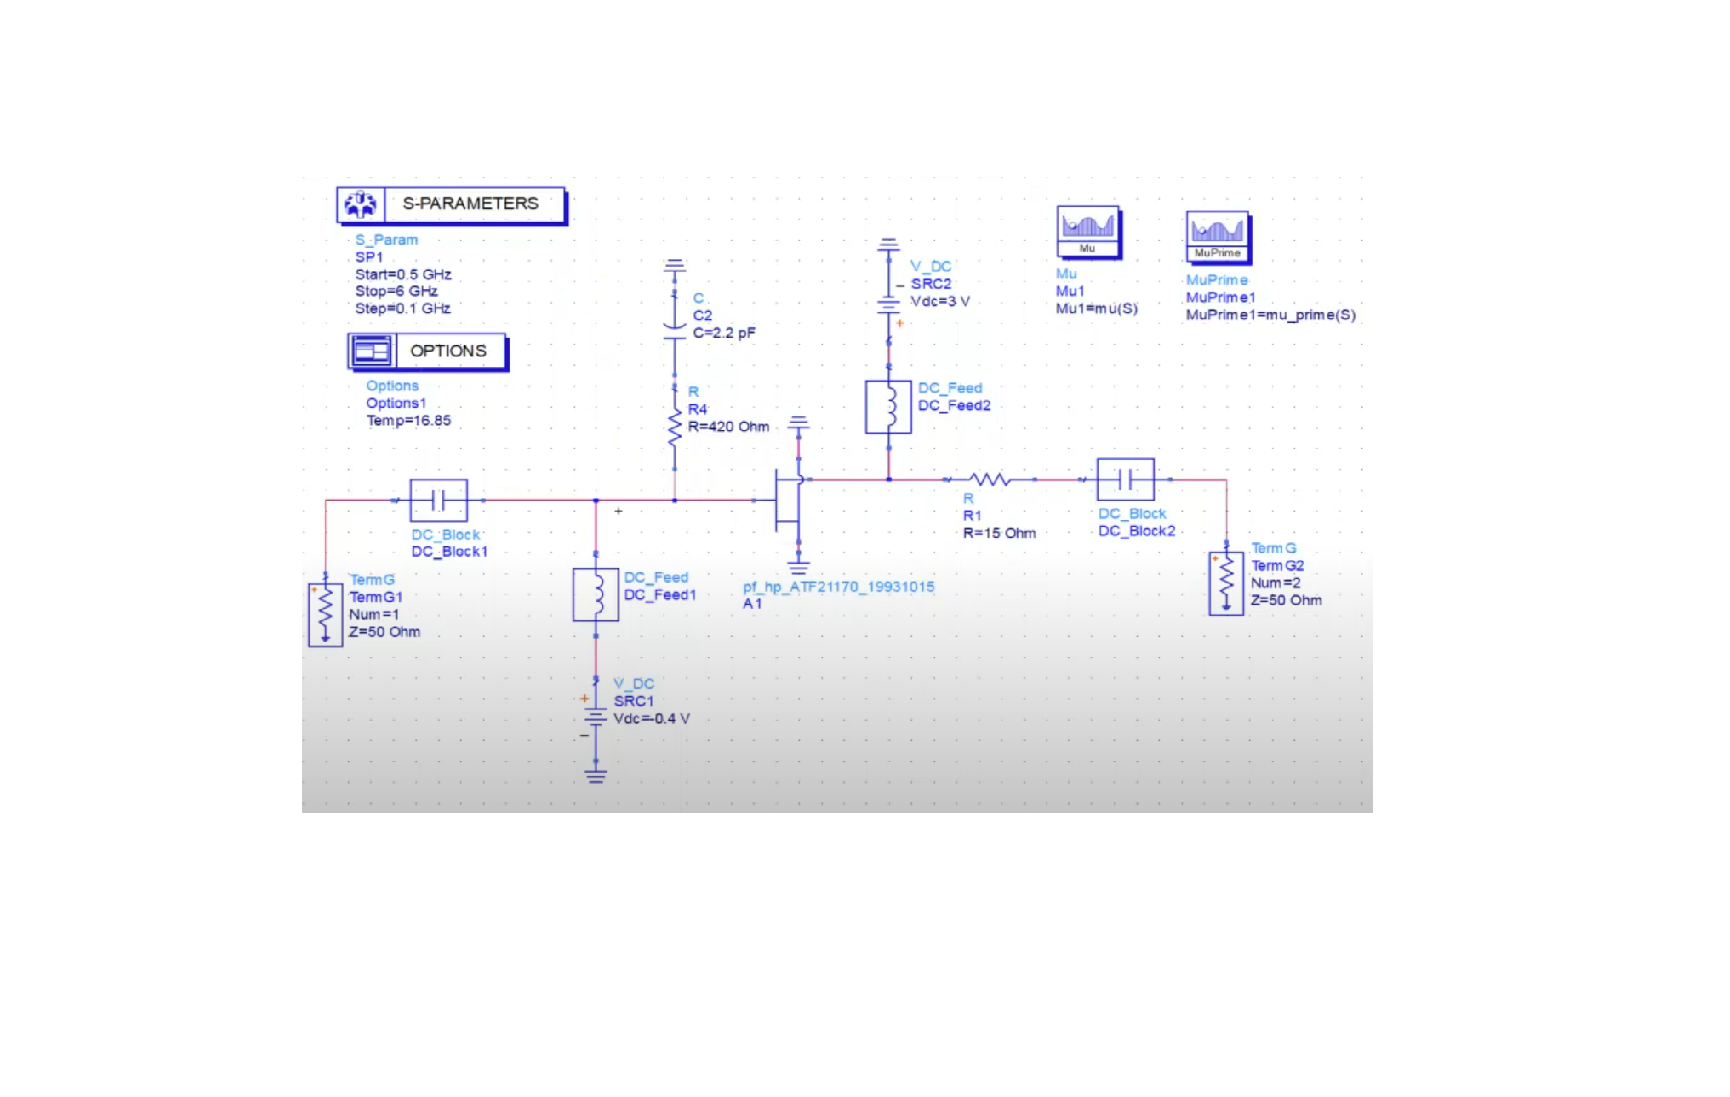
\includegraphics[width=0.8\textwidth]{figures/stability01.pdf}
        \caption{Stabiliy for transistor and amplifier}
        \label{stability01}
    \end{figure}


    so get the stability points vs the the noise value. add series R at the in and out of the transistor dierctly like the R0 but use higher values.

    avoid any noise components at the lna input which could lead to higher NF so the R0 for the stability could be at the output side only to avoid noise but the resistor the lower the better 

    adding the Vds = Vdd for the bias point fot s2p file and also with  Vgs 

    if the design is slightly stable or there  value is lower than 1 by small value it could be solved during matching this is called potential stable but unconditional stability is preferred this for the unspecfied freq range but for the BW it must be unconditional stable 
    als using the feedback is food for the stability and the shunt RC line which is on input side this also can improve the stability 
    but R shunt should be as high as possible for provide a load for the gate of the device the capcitor shuct is blocks the DC from going to the ground throug the resistor 
    with the stability 
    in the dc bias line you can use the choke inductor for the low freq on the video it works for  2,4 Ghz so for our design it will also work otherwise you can use the Mlines circuit snd match it to be band pass filter  means has very low S11 and S22 on the BW and zero S21 as a gain and this means no loss on the BW so make the circuit and match it by the way you are interested on it.
    
    you can also use the capacitor on range pf beside the bias source as blocker and then use the choke inductor nad the resistor and make you measurement on the design.
    as mentioned on this graph for the biasing design also the connected radial stub gives double protection to the what happens on the capacitor besif the bias sourse it like a gnd point to protect the circuit. \cref{Bias0}
    \begin{figure}[H]
        \centering
        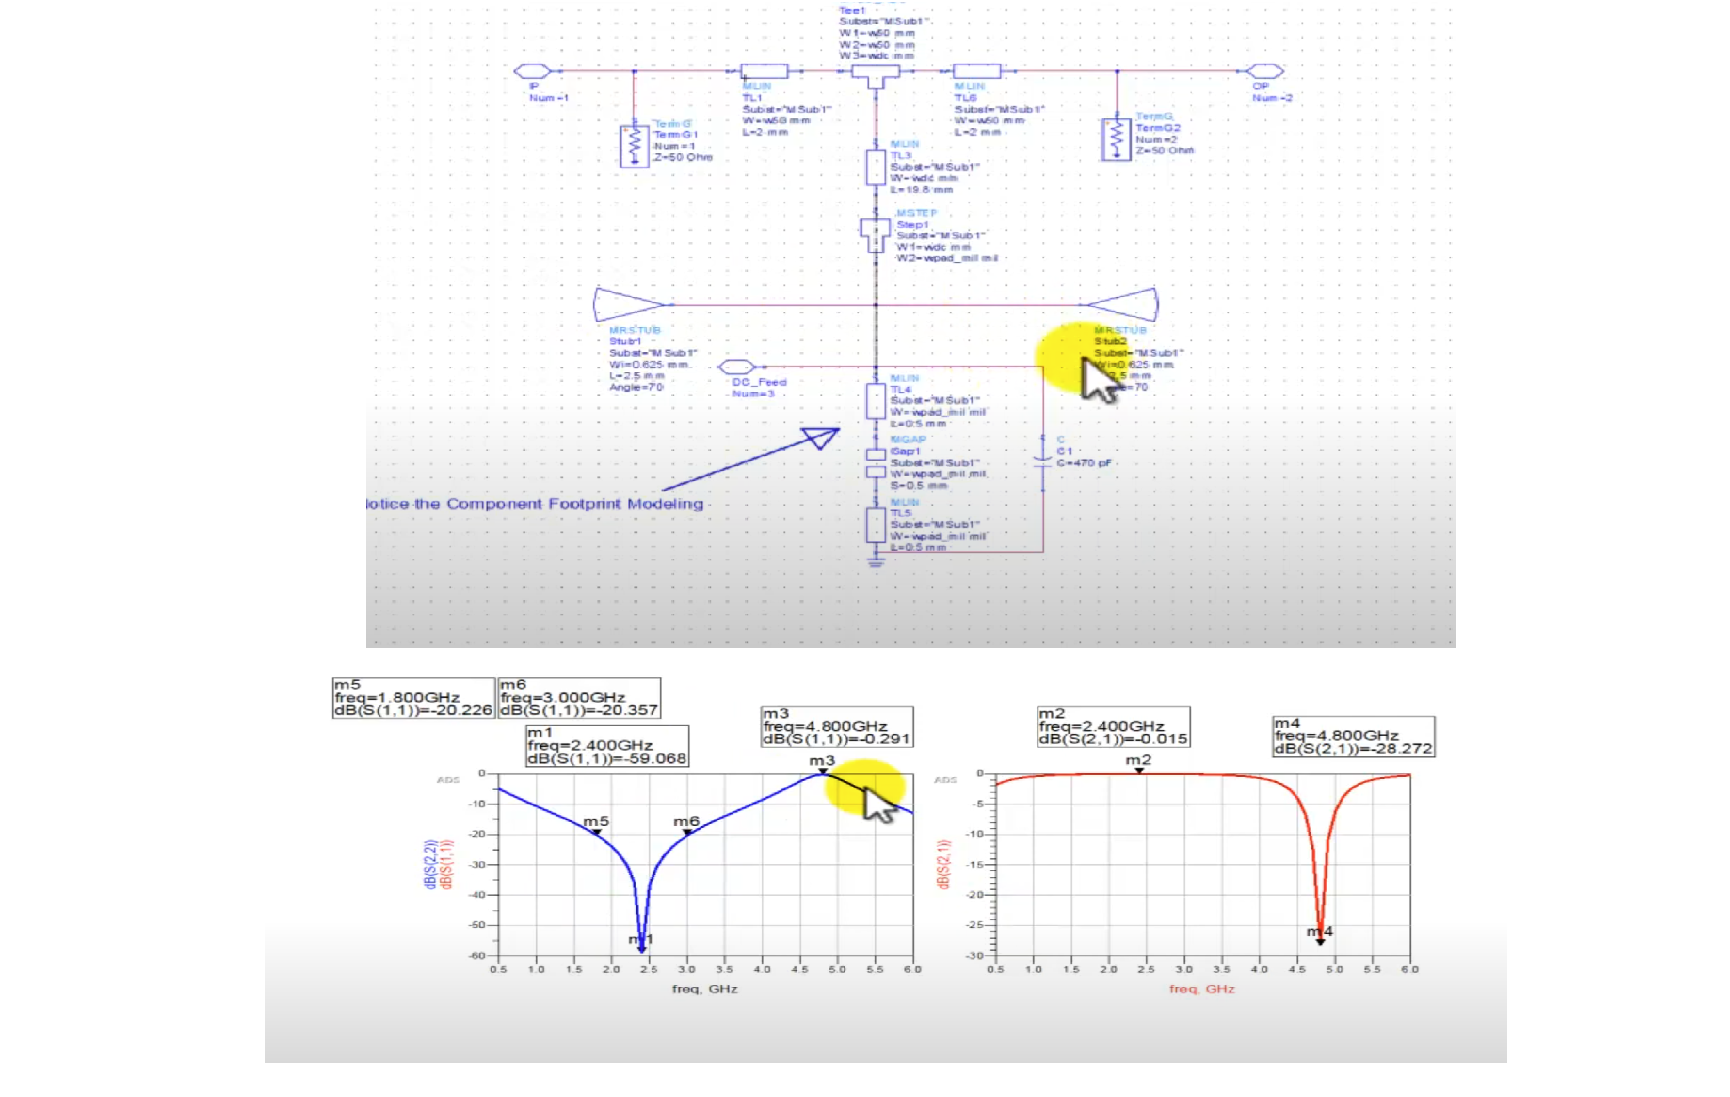
\includegraphics[width=0.8\textwidth]{figures/Bias0.pdf}
        \caption{Stabiliy for transistor and amplifier}
        \label{Bias0}
    \end{figure}



    on the optimization neever try to change the bias componet means the  L chose stay as it is and the Rd just changet the component on the Rf propagation line.


    for the matching at the end to get low S11 and S22  make the matching circuit and make the in and out capactors par to it as you have to use them and shown the figure  beloe \cref{Matching0}

    \begin{figure}[H]
        \centering
        \includegraphics[width=0.8\textwidth]{figures/Matching0.pdf}
        \caption{Stabiliy for transistor and amplifier}
        \label{Matching0}
    \end{figure}

    also just change the compont realted to matching just the feedback and the capacitors and the shunt and series coponent on the propagation line this is an example for a matching  circuits for the componet you are allowed to change.as in \cref{Matching1}
    \begin{figure}[H]
        \centering
        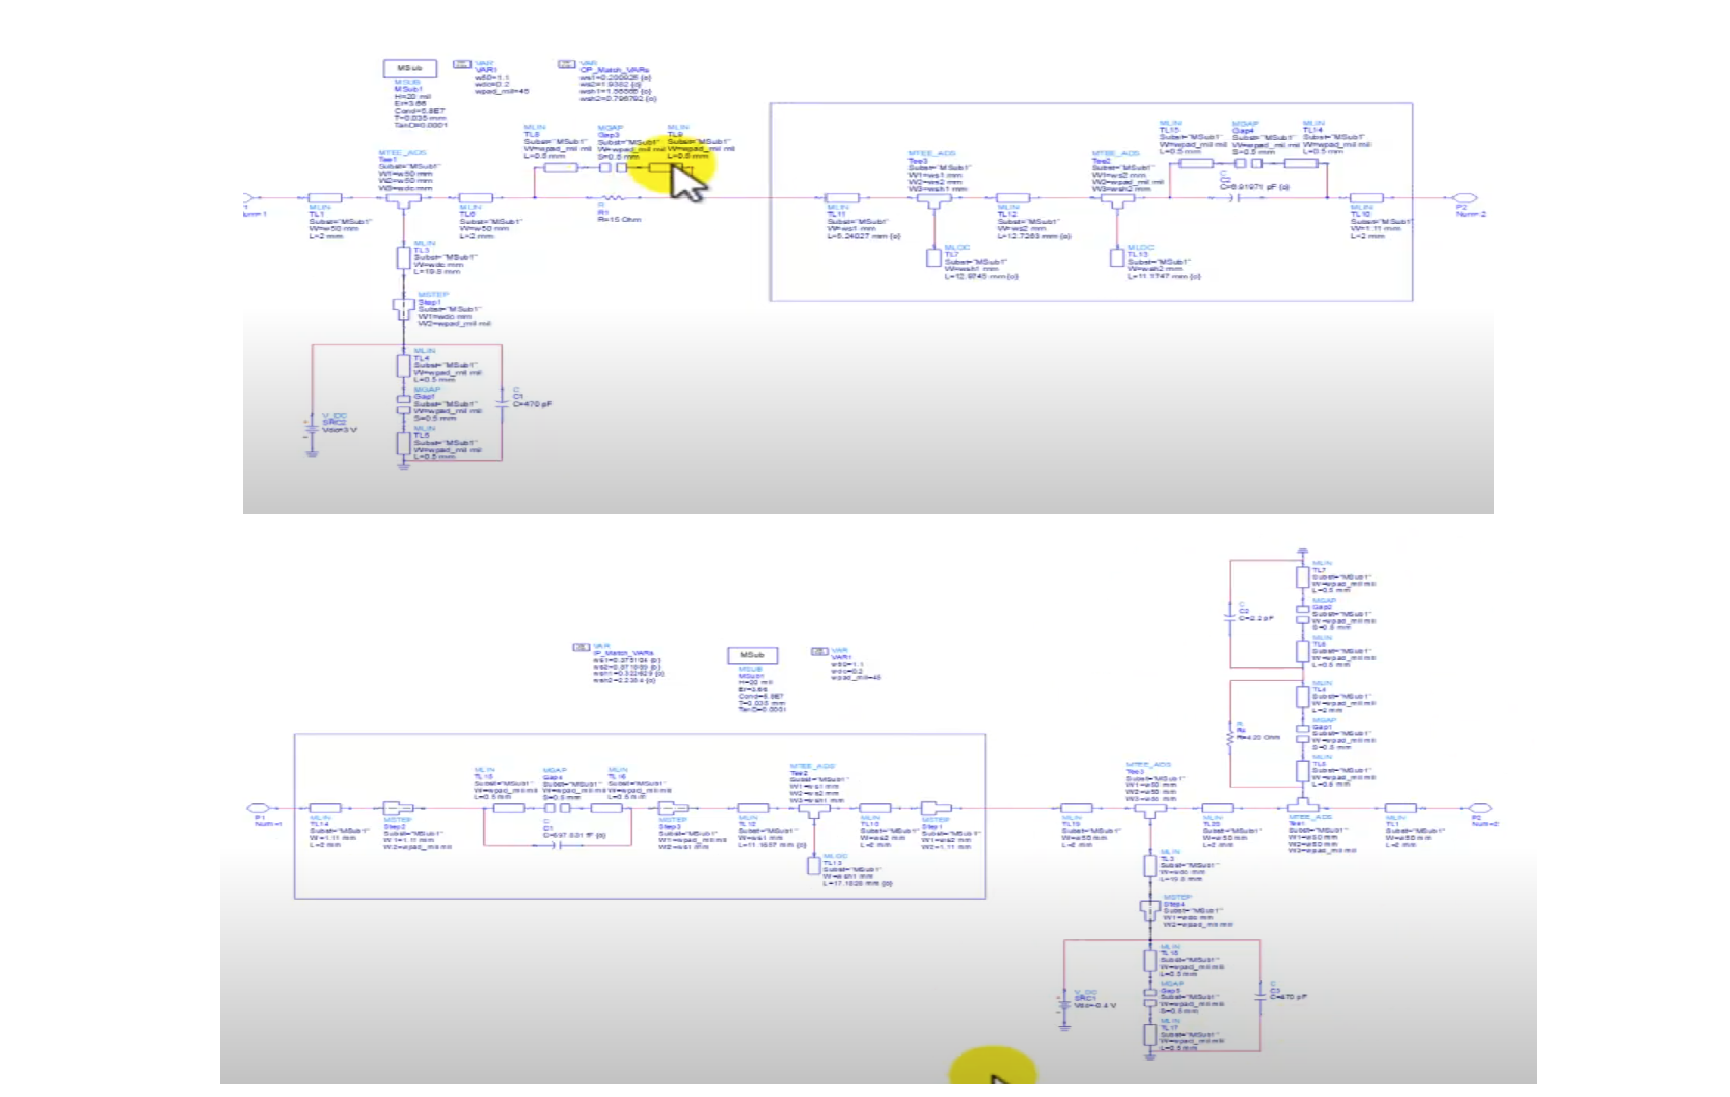
\includegraphics[width=0.8\textwidth]{figures/Matching1.pdf}
        \caption{Stabiliy for transistor and amplifier}
        \label{Matching1}
    \end{figure}

    after every change make full measurment for the design all sparmeter  mesurment and the noise and the stability also the pdc is stable as you are using stable point for the biasing 


the EM simulaton for the layout can be done with s parameters model after you finish the simulation generate  gerber file and fabricate you lna and during EM simulation the amp should be biased with the DC but on the S2p sile it contains the value for the DC point.

for thr p1db point if it should be  higher than 10dbm for example. on the simulaton for the Harmonic balance you sweep pin from -30dbm to 10dbm and mesure the gain vs pin and see where is the 1db compression point. ifit is in on 0dbm check the point also on vout(dBm) on this point and see if it oppose 14dbm for instance it means that out p1db point is on 14dbm  and this means that our design achieve the goal to get p1db > 10dbm 


this is on the RF design 10 by Anurag on youtube on min 50 .

for the noise figur from the steer video saved on Brave browser sou see the gain and Nf tunig graph see it and make it for your design. 
for the matching the stability is most important than it the  staility controlled mostly by resistors at the imput and the output also the feedback  resistor 


the biasing is interested on how much current on Id and the Vgs the mentioned Volt on the datasheet is the Vds and you just apply Vdd so you can control that with the feedback and the Rd you can use just inductors and the current will not changed as it goesout from the source but with thr Rd it might play role the stability and the biasing at the sames time 


using ID meter and the VD metr to measure the IV characteristic of the design make sure to use the marker on the graoh that tells you the value of I and V  at each point


the capactors beside the biasinf sourse is important for the biasing as it  blocks the dc and force it to go to the  design but it does't change the current a<dn the vlolt inside the circuit 



now you can start match before checking the gain as mathcing over the spesified BW is modt important than getting the gain. so the blocking capcitors can be part of the match circuit 

smith has a good notes as mentioned on this grapg from Rf design 6 by Anurug \cref{smith tips}
\begin{figure}[H]
    \centering
    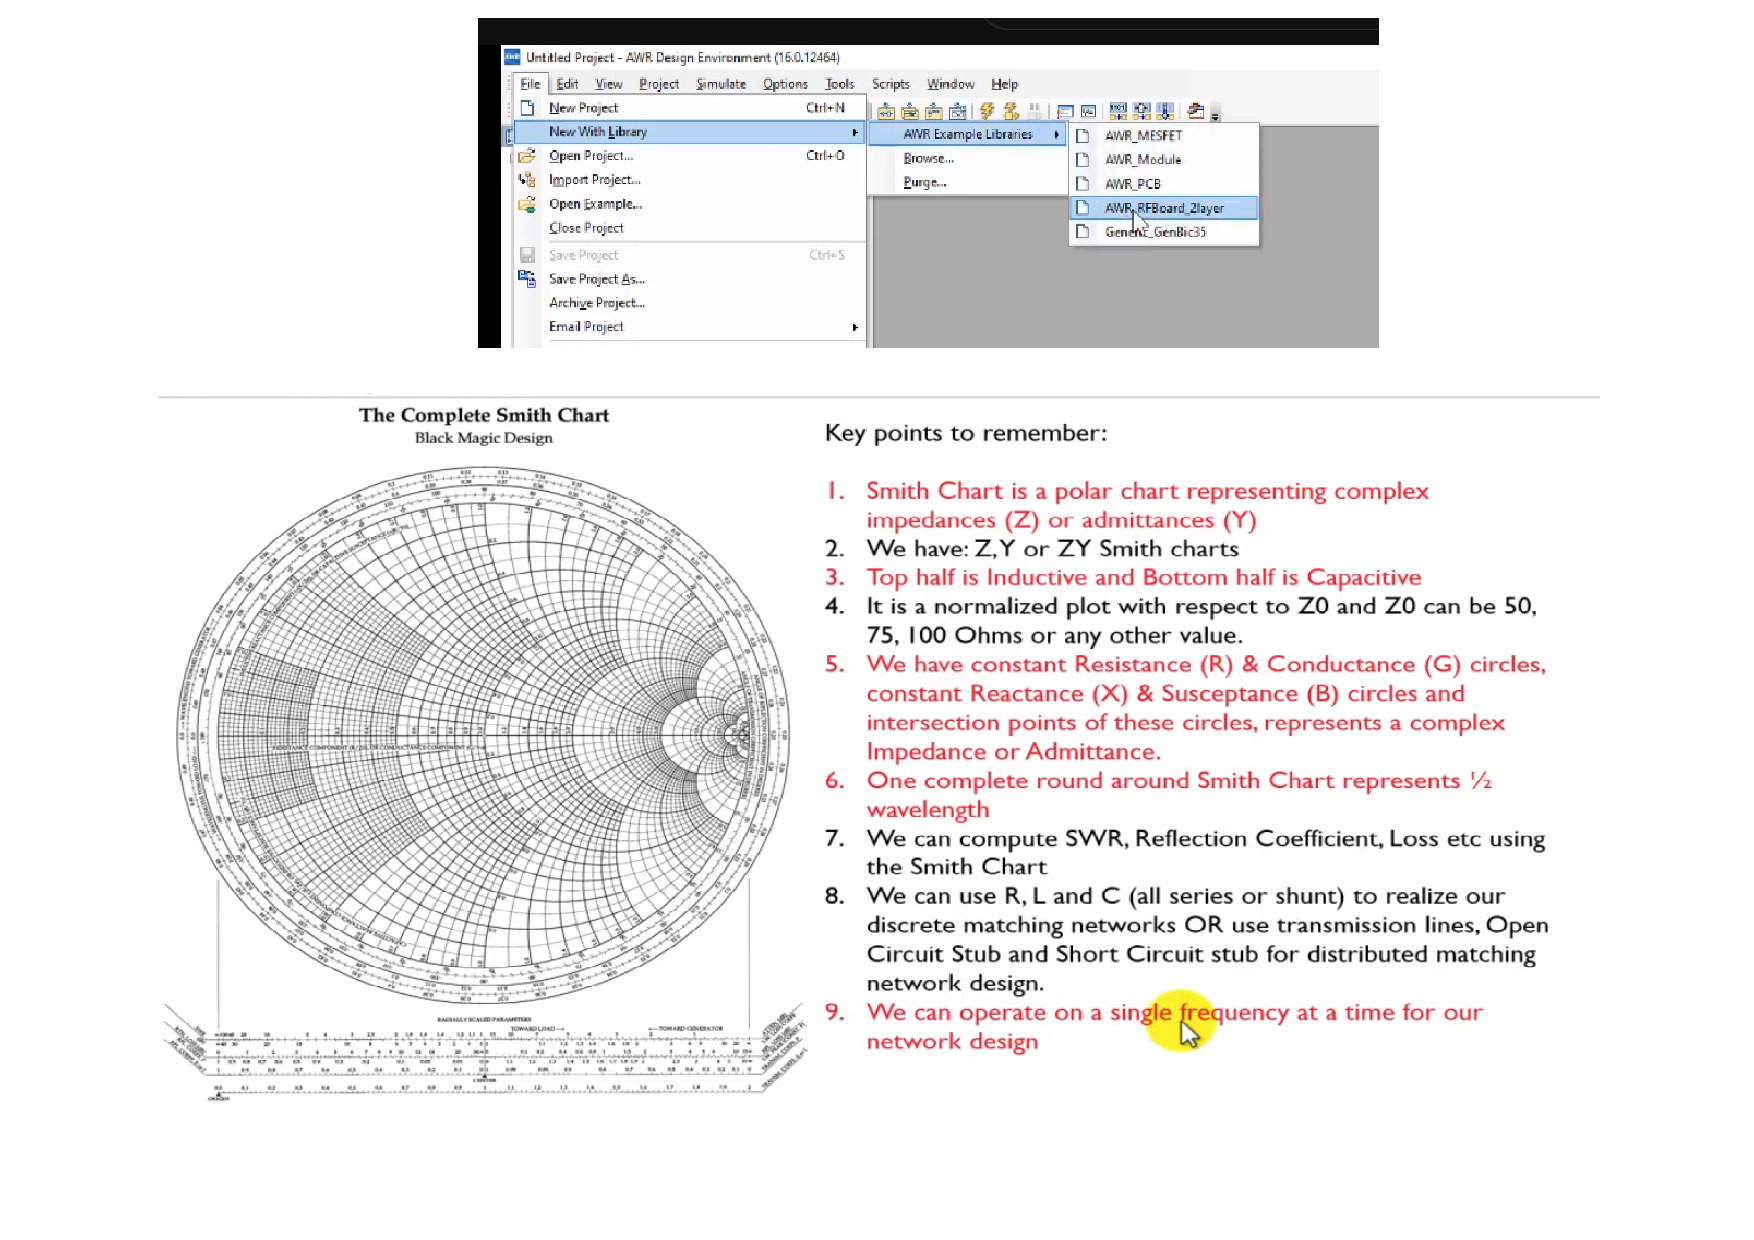
\includegraphics[width=0.8\textwidth]{figures/Anurug rf6_1.pdf}
    \caption{Smit important notes }
    \label{smith tips}
\end{figure}

you can make the matching circuit outside the blocking capcitors

start with measure the Zin on smith for a spedifed freq as smith can work in single freq only check the in or the out impedance and match it with a 50ohm or any other soure 
for example if the inpput of the transistor is 500 ohm and the  sourse port is 50ohm  now you will need to match 
Zin can be cosidered S11 on complex units this might be agood idea for SNSPDs 
this for Z11 and Z22 


matching between two point is by finidng them in smith and then move one to the other point by the LC circuit this means that the interstage capactor between the two stage LNA 
may be will no be enough for the matching between the two stages . for example if output of stage 1 is  $10+j*50$  and the  input of the  2nd stage is  $50+100*j$
so show the two poitns on smith and then move one to the other no need for 50 ohm matching here.

on matching you could add the two shunt or series beside each other but preferred to use one only. this point is important for our design due to the two component at the input amtch side if you don't wanna use a R and C .
all matching network are simply filters between unequal termenation on each side 


\textbf{Broadband matching}
here we use the q circles method or called the $q factor = center freq / BW $ then you will see a another graph at the middle of smith. as shown on \cref{Anurug rf6_2} 

Q factor is $1$ if the  you wotks on single freq  higher q number means BW lesser and lesser and the circle increas 
the idea here is to make a smith inside the smith and you are only allowed to move only iside the smaller circle so every time you wanna change the directon you need a new component so the Match circuit will be  many component not just an LC circuit as on the the graph fir 3   \cref{Anurug rf6_2}  

\begin{figure}[H]
    \centering
    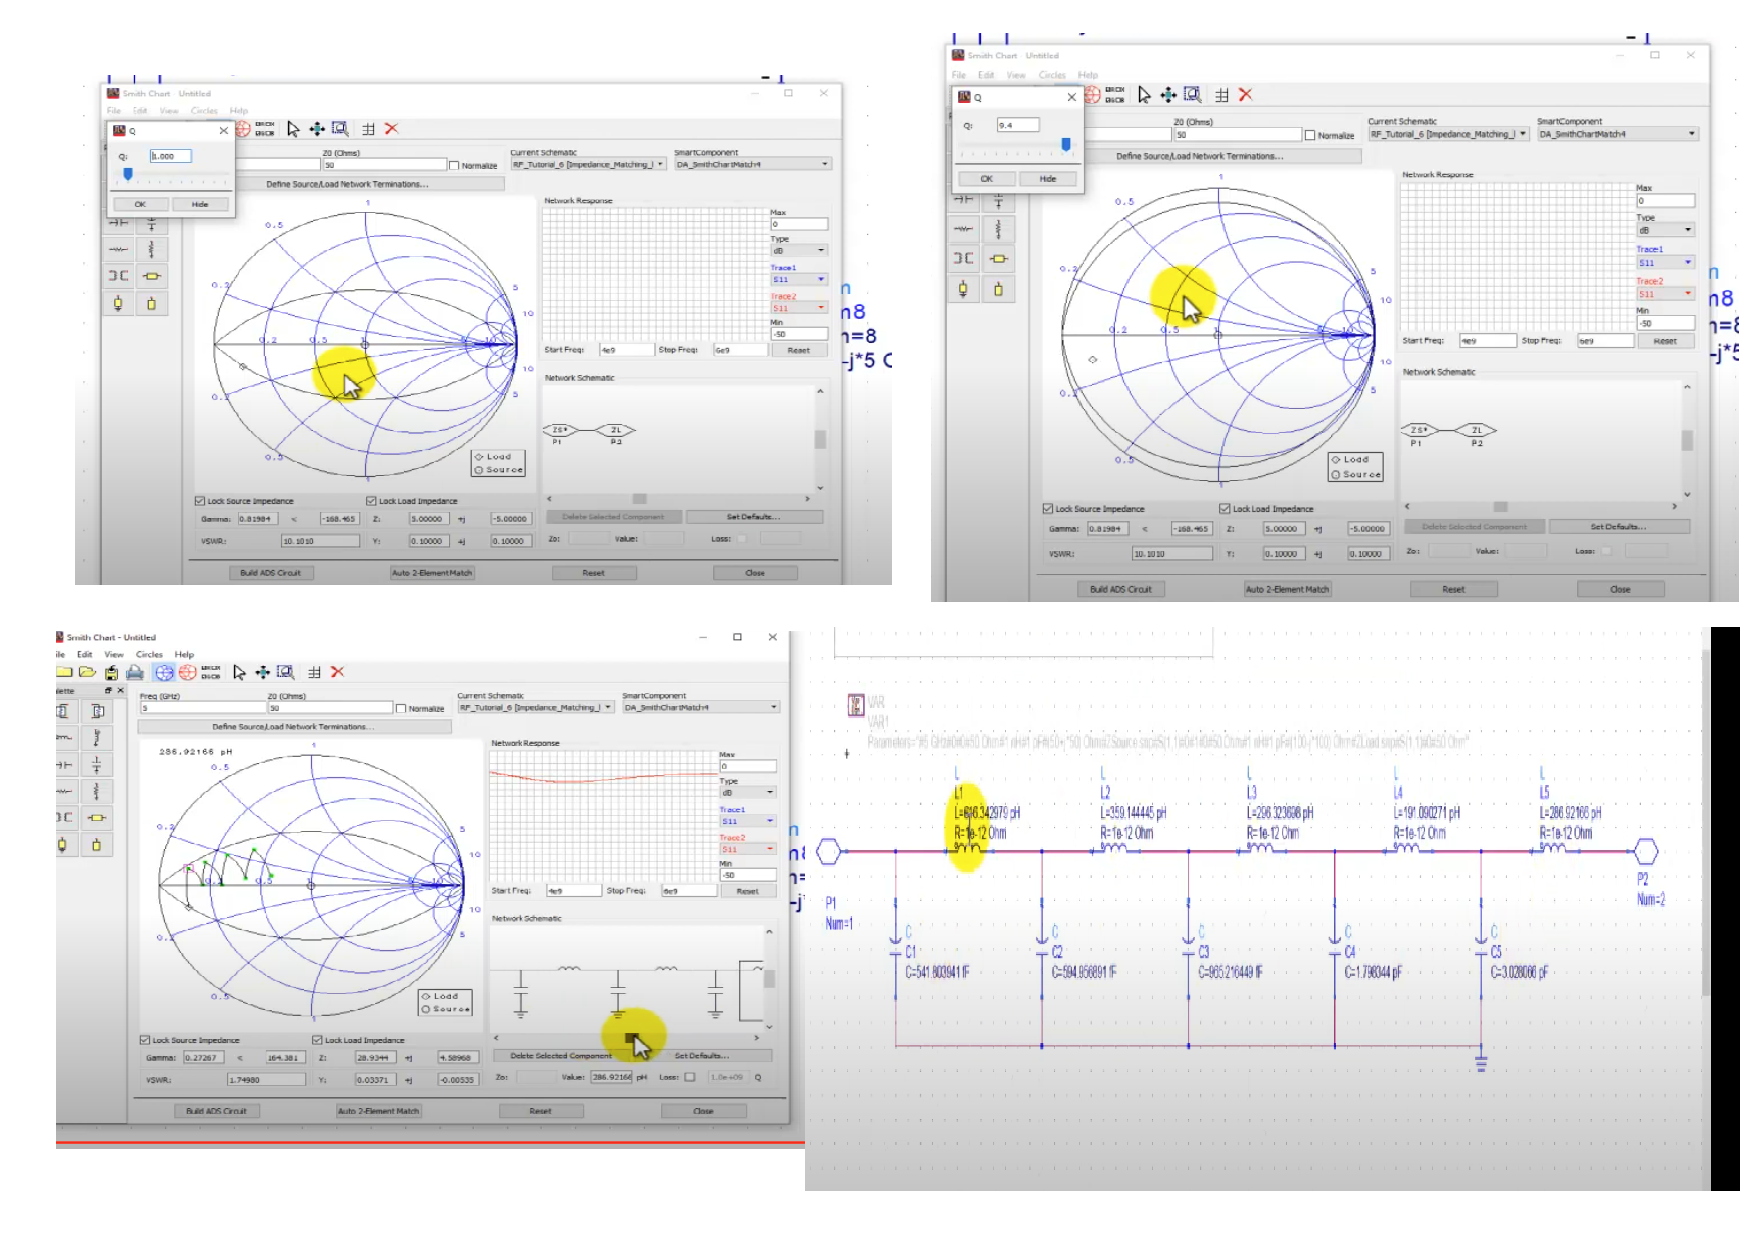
\includegraphics[width=0.8\textwidth]{figures/Anurug rf6_2.pdf}
    \caption{Smit important notes }
    \label{Anurug rf6_2}
\end{figure}


but the whole circuit now is ideal component with 0 ohm resistance means q factor is very high 
more BW means More indertion loss or S21  and gain but the large amtching circuit is will add anoide figure on the LNA 
on the  Power amplifr this might eat he output power if this is the output matching circuit.
another point is the Broadband mactch will change the load and the source impedence during matching so this needs some tricks to deals with it.means the source and load impedance vary with the freq as you work on BW 
Impedance mactching importance \cref{Anurug rf6_3}
snp is also called s2p files. 
one of smith chart is it works with  only one freq and all other factors will based on it .now you have to use the q factor circle with the center freq ans then dfine the in and out impedance on smith chart and the add the lumped elements to match over the Wideband . 


\begin{figure}[H]
    \centering
    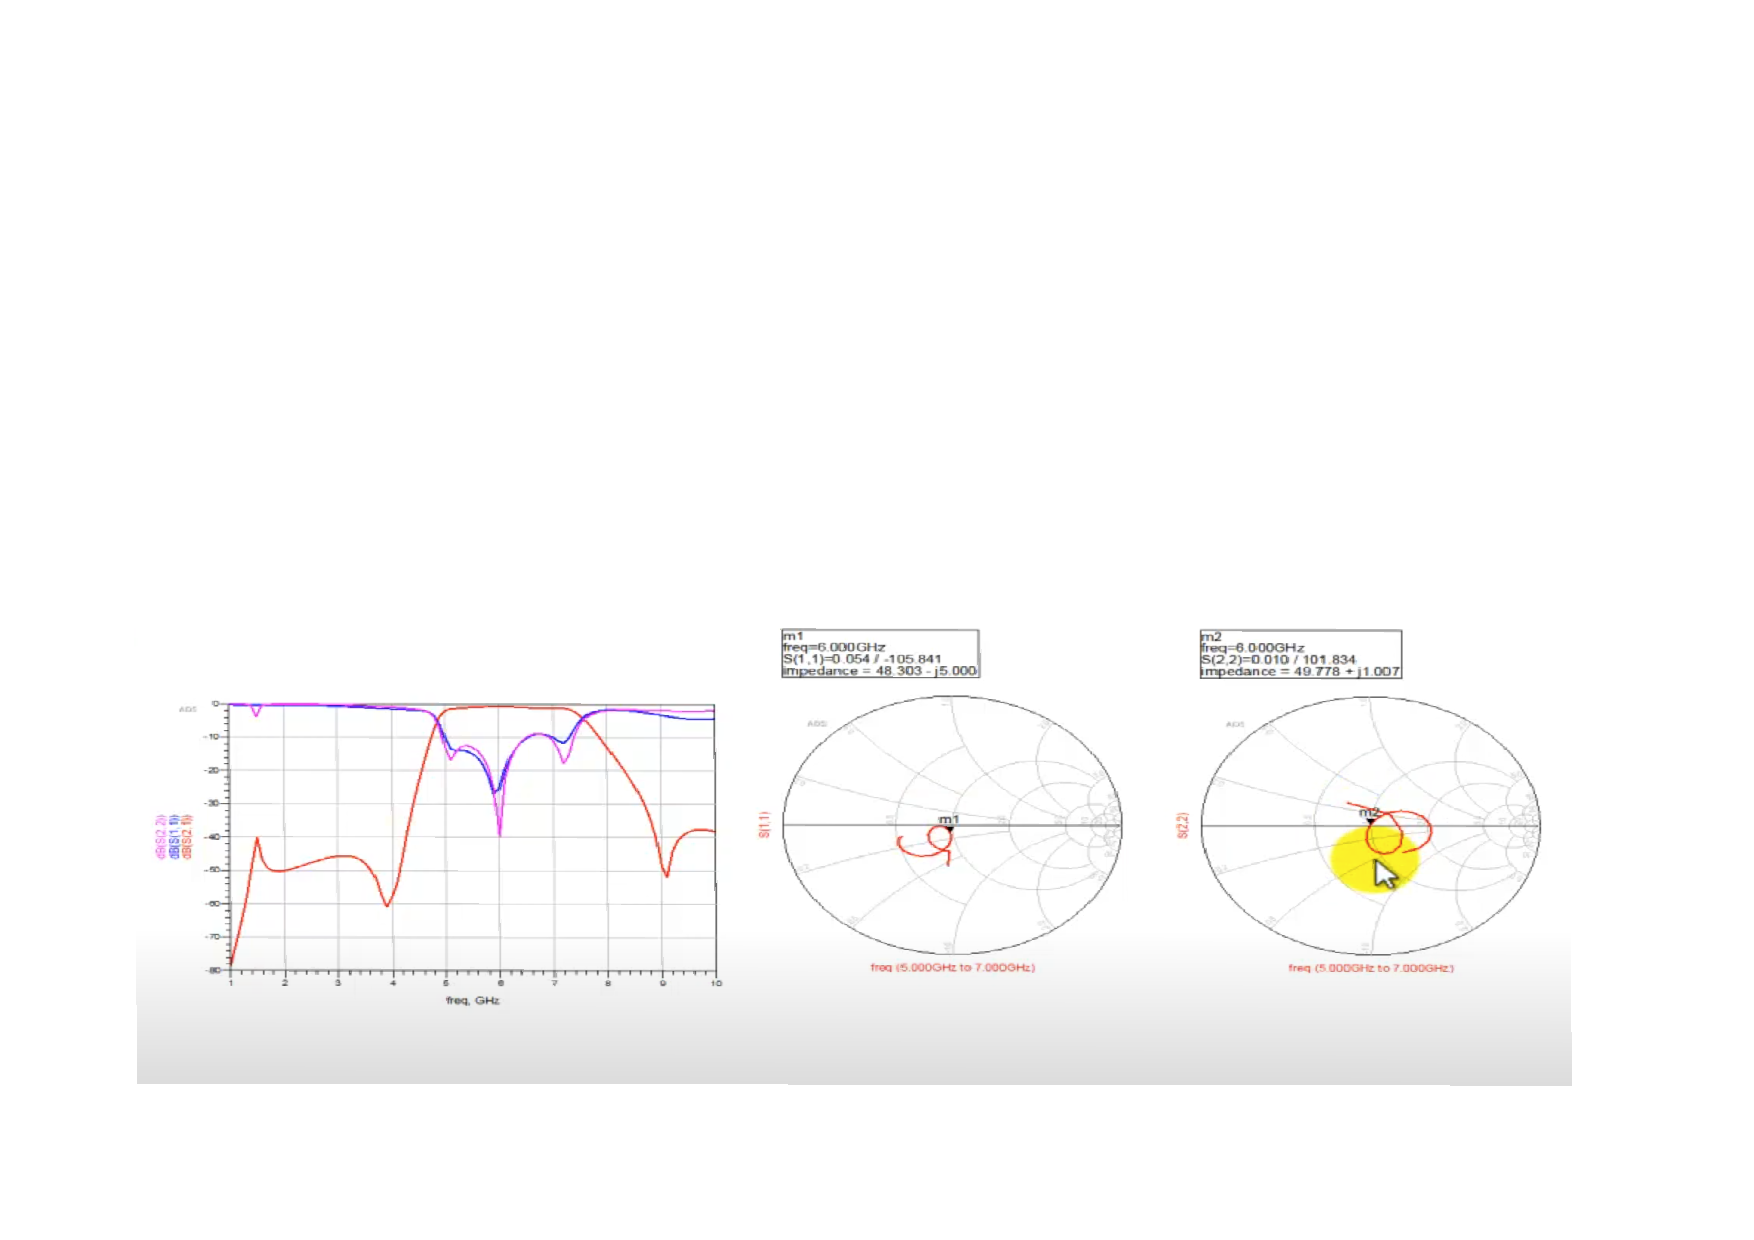
\includegraphics[width=0.8\textwidth]{figures/Anurug rf6_3.pdf}
    \caption{smith after widebend match the matching is not as good as ecpected as we didn't consider the freq dependeices on the BW }
    \label{Anurug rf6_3}
\end{figure}
 

the frequency dependeices can be solved after matching with tthe optimization tool as on AWR by define optimization goals.
on the optimization for the inductance it has L and R , do  you should chose just L and C on the optimization tool no optimization for the R, so the wide band match is done for the Center freq but with the Q factor circuits, then apply optimization to get the best result.


\textbf{Match Cascade}
this is very diffcult to measure the in and out of the two stages sepertly as the are connected and we can only measure the  S11 for the 1st stage and S22 for the 2nd stage,
and to match we need S11 for the 2nd stage also S22 for the first stage and no port connected for this measure.

threre is a tool called SP probe with 50 ohm match at the two sides the pic define the proces \cref{Anurug rf6_4}
it has left and write probe L.S11 is S22 for the 1st stage and R.S11 is the S11 for the single stage. for the sp probe you need to define you freq range. also check what other measurment can done with Sp probe as on the fig \cref{Anurug rf6_4}
this means you have defined a port inside the design 
also you can use the impedance match tool on ADS it show the types of matching method by filters with LPF, HPF and Band pass filter.also with thr transmission lines 
and connect the network as on the  figure 

and aslo the match network topologies might be Diffrent. the topologies can be optimized and generated by impedence match utility tool on ADS on lec 7 with Anurag.

\begin{figure}[H]
    \centering
    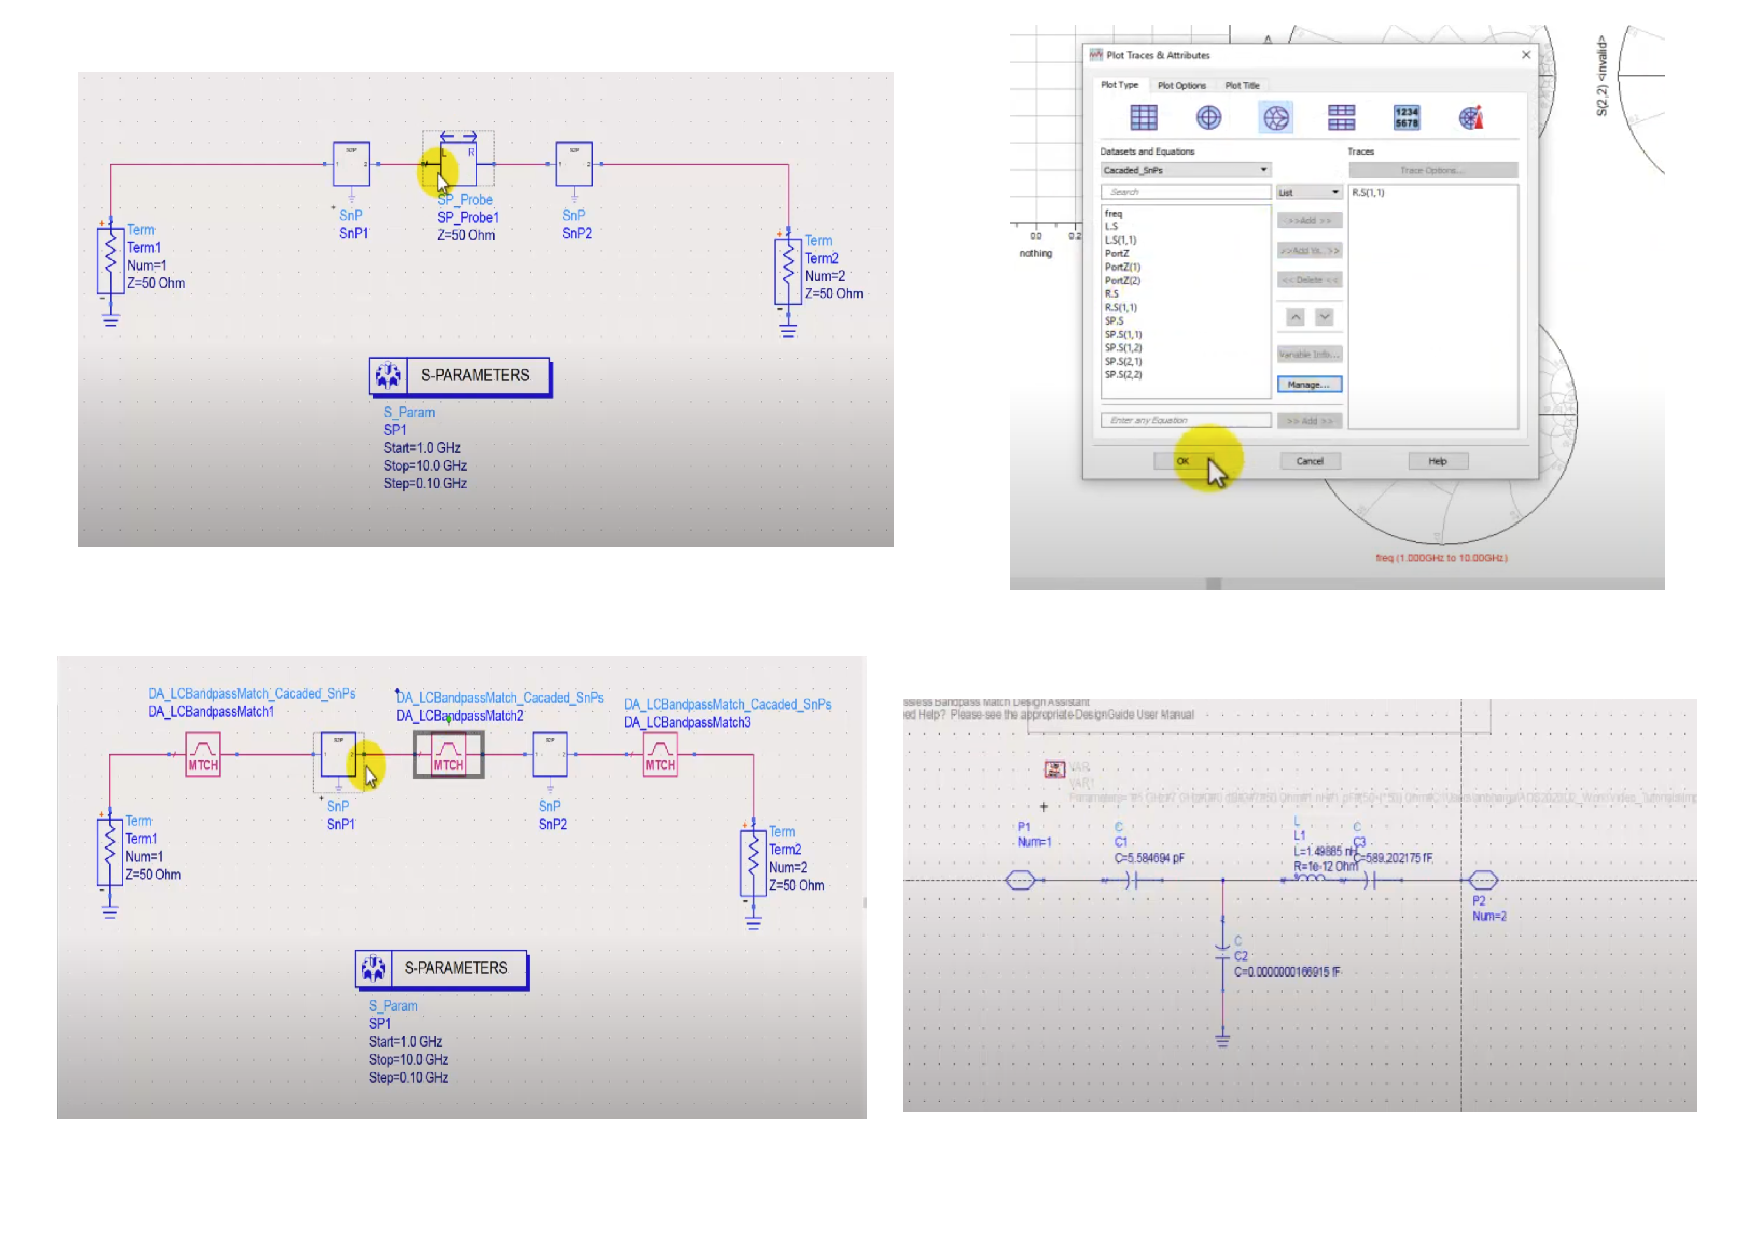
\includegraphics[width=0.8\textwidth]{figures/Anurug rf6_4.pdf}
    \caption{smith after widebend match the matching is not as good as ecpected as we didn't consider the freq dependeices on the BW }
    \label{Anurug rf6_4}
\end{figure}
 
also after Cascade matching you need opotimization due to the freq dependeices 
the component that stops during optimization is because it reach the limit of the measur 





\textbf{Mtching with Tlines}
tline normal,  is jsut ana LC netweork, default Impedance is 50 ohm , increse the impedence of the line makes it more inductive, or it will behaves like an inductor on smith chart , bbut tline with higher impedence or lower is no avilable practicaly, higher impednce means very thin line, capacitance will be negligable so the tline is an inductor.


openstub,  will behaves like a capacito. so if we leave the line on the pcb open it is like a capacitor, for the open stub if we decrase the  impedance it will be more capacitive,means wider tline, 

on the txline calculateot the  higher the impednce the lower line you woll need means smaller W and Length. most of the pcb is 0,2 mm width, W_max is 3 mm but with no upper limit,


the input amtch is SMA  sourse and  input for the transistor load  these is the two sides for the input matchso mostly the output of the match circuit should be loaded on the input for the follwer component 

for the tline after you make you design there will be the problem of variable freq with the component during match so we need optimization but for the tlines we optimize the El on not the impedance and the center freq still the same.also you could optimize the resistance but with adding constrain for the values.

during the optimzation you if some component say that it reach the limit defined on the  constrain you can change it and continue the the optimization,

to add the important tools from the device you can define your own hotkeys from the hot key tools bard and fine the needed tools. 

after you work with the tlines which is optimum you need the physical lines with the MSUB  like the lines on the PCB, on ADs there is a method to convert the tlines  to Mline means you add the characteristic of the tline the impedance and El and F0 and then on the lineCalc open your MSUB it will converted to a Mline with length and width, on the line calculate tools use send and update icons tools to modfy the component as on fig \cref{Anurug rf8_0}

\begin{figure}[H]
    \centering
    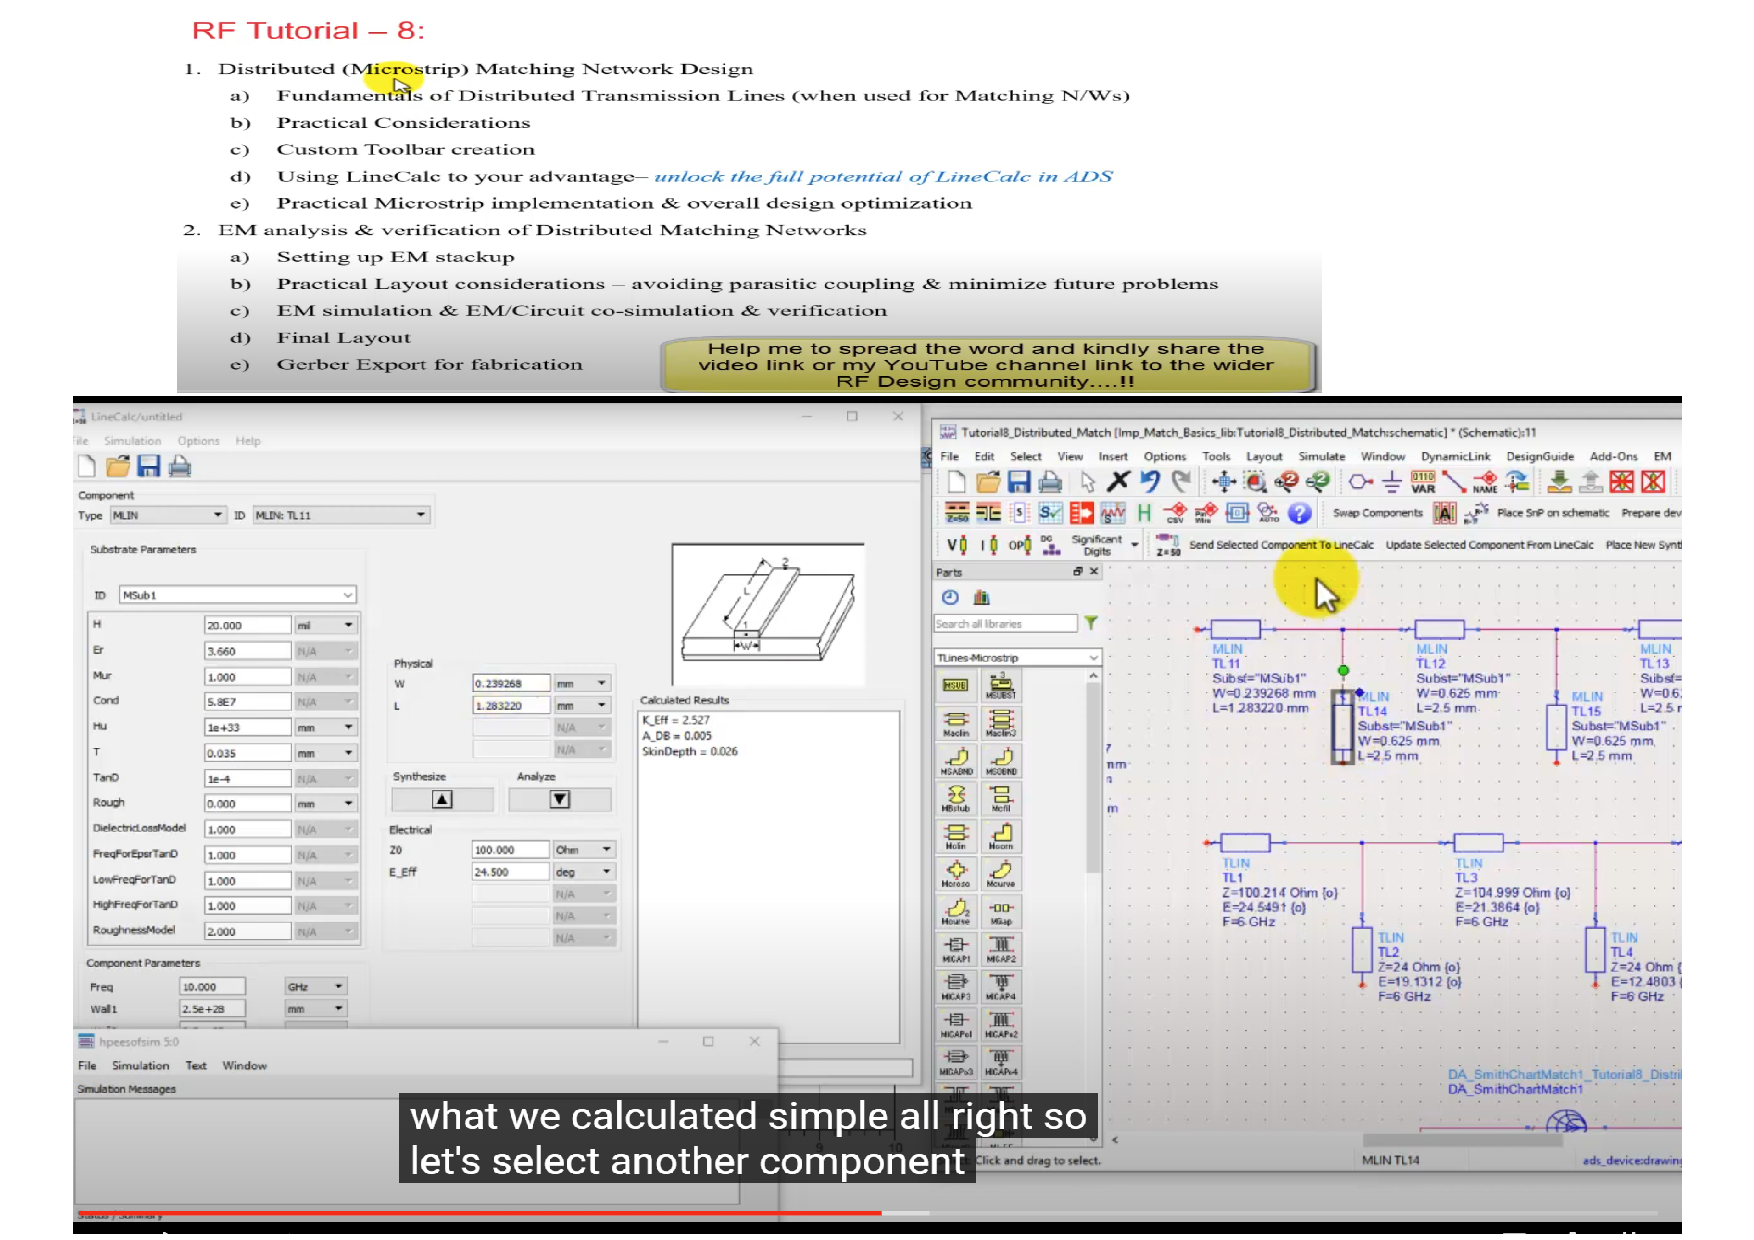
\includegraphics[width=0.8\textwidth]{figures/Anurug rf8_0.pdf}
    \caption{Tline to Mlines converter on ADs }
    \label{Anurug rf8_0}
\end{figure}

the convertion is  done line by line for all the component, also don't forget to add junctions for the lines connect on T shape , and slo there is junction for lines with Diffrent lengths meand jsut 2 lines nnot 3 as on the T junction form, and alaso there is for connect more that 3 lines on the pcb.
after changing all the tlines you need also optimzation tools but preferred to make all the parameters values on a equation form to save tthe shape of your design,

on the optimization if youe see a good result you can stop the simulatoin and update yoour  design , 




\texzbf{EM simulation}
at the beginning generate the layout of the design and by seeing the footprint for all the component, the Mlines has there own footprint, if a component with no footprint add a footprint for it from the software library, 
if there is dicontinuty on the layout this means there is a mistake on the design lool for the component and correct it then optimzation agian for the design as any chages might make you lose the point of matching, this means that if increased line as opne stub or short might means add a component and this  will lead to mismatch over our point. 


then add pins for the input and the output of the design, if you looks for the stackup you will see a 3d view for the Mline and the substrate you prepared is imported ont view so can see all the connection of the design, so for the EM simulation you need the pins and the stackup 


for the EM creation is by make the EM setup, chose the EM simulator to use from Momentum Microwave and FEM and Momentum Rf 
for the  voideo RF 8 by Anurag this by he uses Momentum Microwave , 
see a tutrial hoe to set it up 
aou make the EM model and make the co simulatio for the design and circuit representation 
means after you make simulation for Maching circuit you make the the layout form and then connect the other components models and make the Em ssimulation agian,
aftr EM simulation you see the same measurment you did for sparmeter simulation
and check the result does it still the same or not  co simulation is Em simulation and it is imulatiion for the real design.

thef inal layout after simulation means making the final pcb layout draw it and define the size and make the holes and the width of holes, 
when adding the holes you can make a grid of holes with rows and colomns and then add it to the layout, 

at the EM simulation again after the design is finished make th via holes lumped to not consider it on the simulation which will save the simulation time and memory of the device,


then export the gerber file of DXF for GTs fro ADS  chose gerber/drill format then open it after it is exported, 
gerber file will show the final pcb layers, 
the gerber file can be changed for the txt editor viewer 





\textbf{NI AWR manual PCB layout and Gerber + drill file generation}
gerber files is about a files for every layer alone, you can download it from internet as zip files.
stackup of the design means the matirials characteristic for every layer. 
from options chose layout options 
control the grid spacing 0.5 mm 
and layout fone  0.8 mm
from layout default beisde the element tab you can control the layers add new layers like add FCu layer and add also BCu add the layers names as you know it from kiacad 
after you add the layer open the schematic and then from tools  open layout files then start control the layers you  can draw it or use the footprint for the component used
after you finish from the layout menu go to the default and chose the export gerber file and modfy the name and save
then form scripts icon chose layout then  chose  ecport pcb drill gerber 
you will have a files output then you can open the gerber file on other gerber viewer as gerberview.exe
after you open it the files on gerber has defined extenstion for every layer you can search online for that 
so change the files ectention and save it then you can send to a company to fabrication process 






\textbf{Simulating power}
change from port properties the power port to souce it will show 0dbm which means 1mW 
on the figure \cref{power1} you expect two input p2 and p3 is 1mW so p on p1 should be 2 mW 
on the meaure use PT the total power in dbm or in mW 
you see less than 2mW 
on the curve you look on the middle valiue it is 1.8 mW means there is loss or reflections 
and also if we add 4 sources it show less than 4mW 
so important point the output port that you take the power from it it will be normal port and the others is sources
if the results is not accurate on project option you can change the interpolation or passivity  from  linear to interpolation 


\begin{figure}[H]
    \centering
    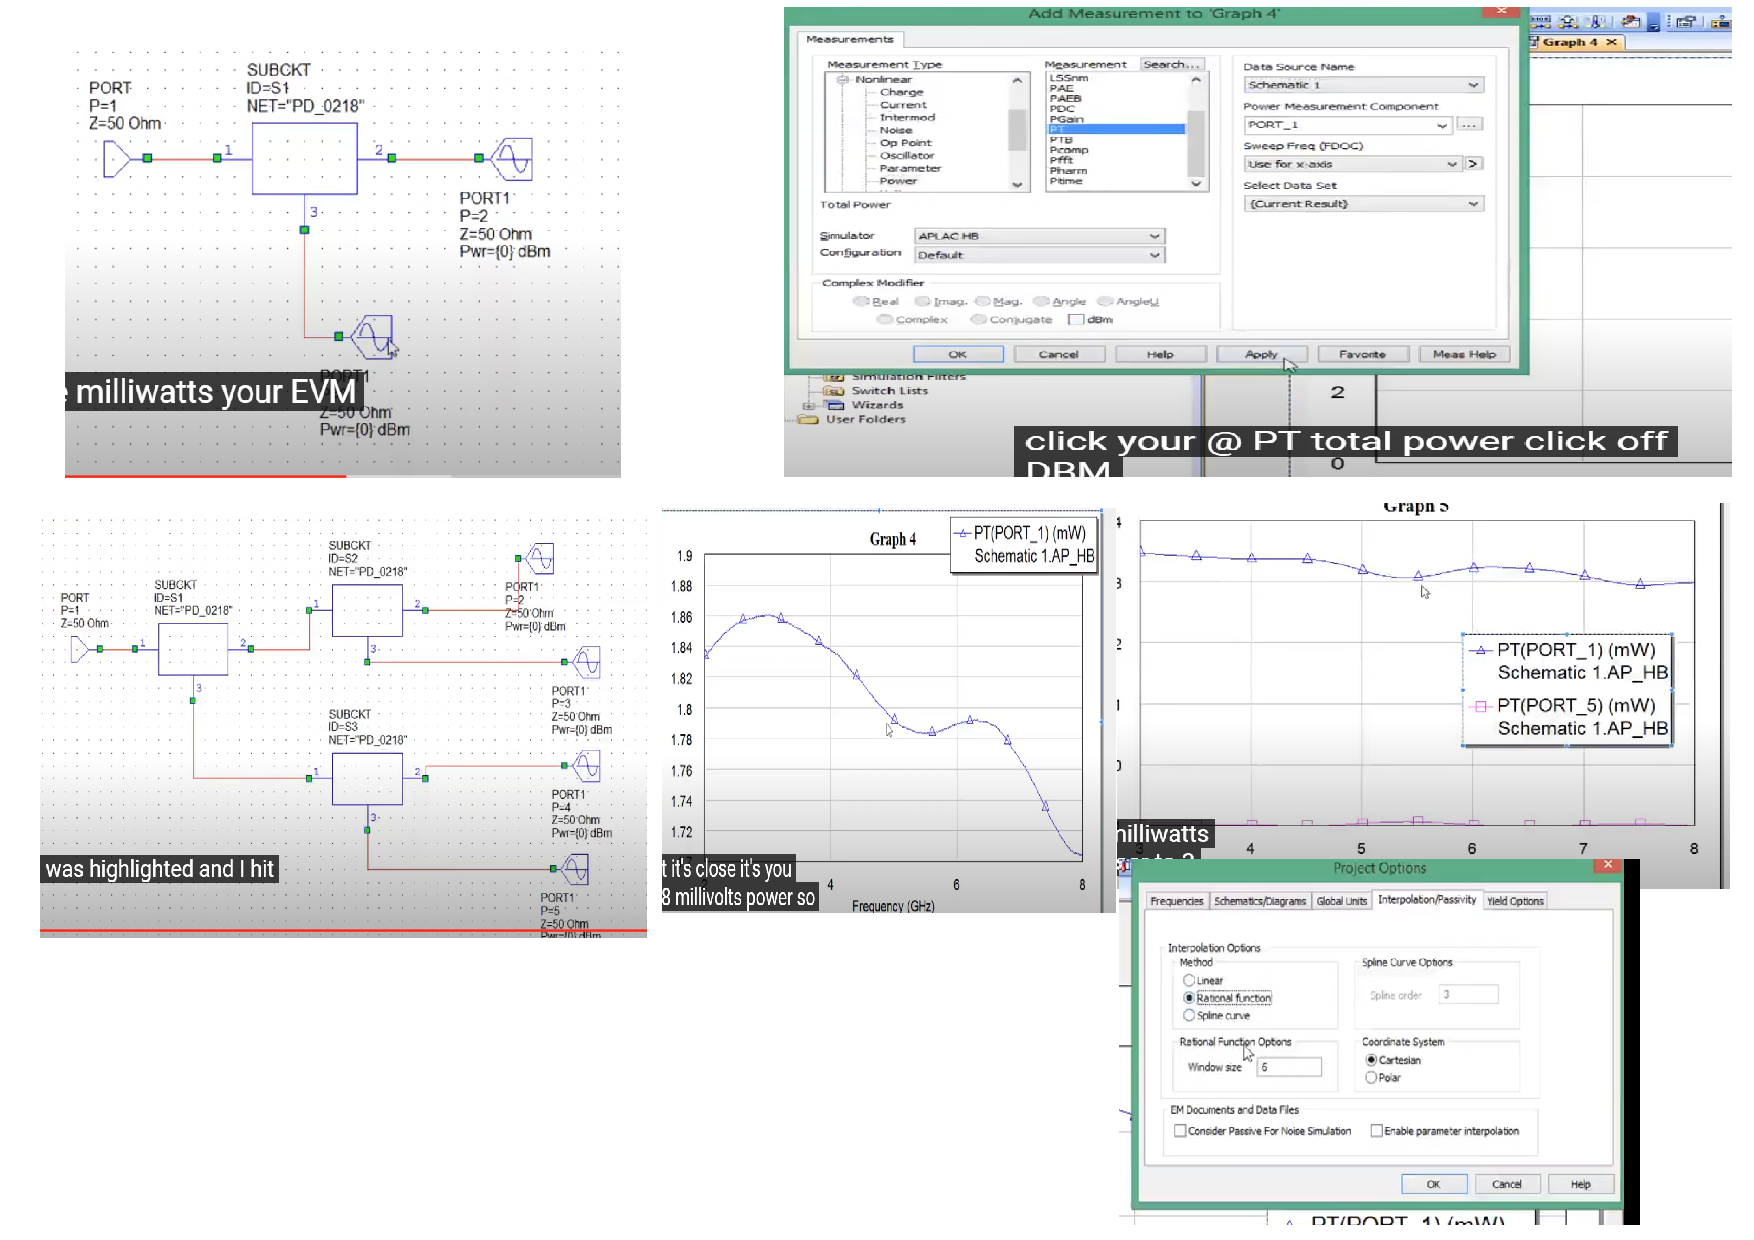
\includegraphics[width=0.8\textwidth]{figures/power  ports 1.pdf}
    \caption{Power measue on AWR schematic and graphs from s parameters}
    \label{power1}
\end{figure}



\textbf{EM structure simulation  and optimization on AWR}

after optimization on the awr from scripts create stackup this should be  done during the schematic window is active
after you pres create stackup 
make the gird 0.1 inch  then change the layer 2 matirials to MT from EM layer mappinng after press on the stackup.
and the line type to MT on the defaults after adding line 1 and remove it after you make the changes.

then enables EM extraction from the  from clik right after chossing with shift key all the component without the port 
then right click properties then Model extraction enable it by check mark.


then go to the layout from the edit button above click select all the snap together 

then from options_then layout options  on snap together part make it auto snap on aprmater changes shown \cref{Em1}
then go pack to the extract block on the schematic right click then chose add extraction thsi will all file on EM stucture  on project left menu .

after you create EM ectraction on the layout window there woll be uppper right icon called show 2d map 
this after click show the layout with the squares inside it. for me it doesn'T change may I did somthing wrong.

if you want simulate the em extraction on the block shown on the schematic press on it all the component will  change to red.

then press simulate, this will  take 5 mints at least tot give the results 

\begin{figure}[H]
    \centering
    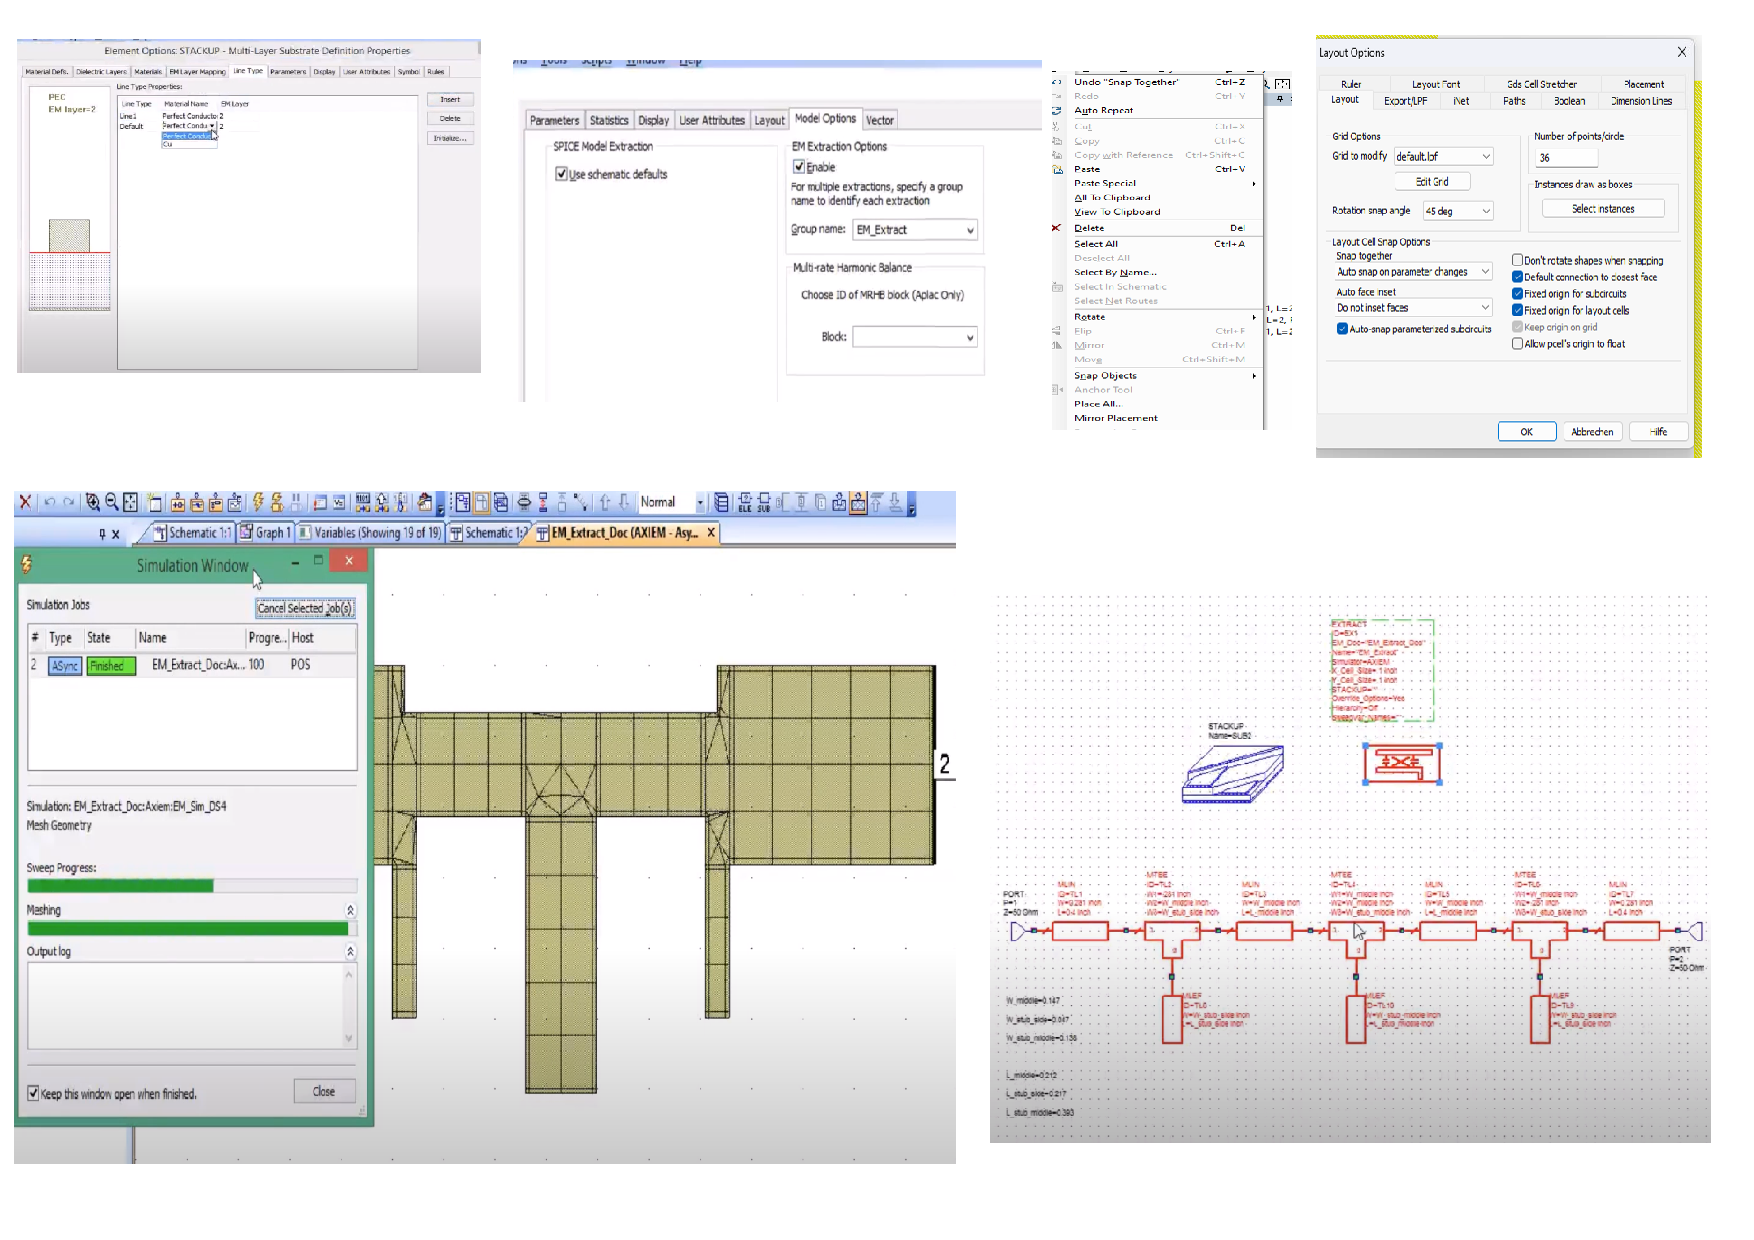
\includegraphics[width=0.8\textwidth]{figures/Em1.pdf}
    \caption{Power measue on AWR schematic and graphs from s parameters}
    \label{Em1}
\end{figure}

the EM structure simulaiton is called the structure with the closed form models and if the schematic is the same as the EM structure means the simulation is nice.

after the EM simulation make the optimzation again but now change the iteration to low number to prevent long simulation and also the simulation method can be changed.

\textbf{another EM tutorial}
on the global defining make a stackup from the substrates on element.

on \cref{Em2} follow the picture to make the design of a stackup manulay on the schematic on global definetion make it and from the properties make these changes.
\begin{figure}[H]
    \centering
    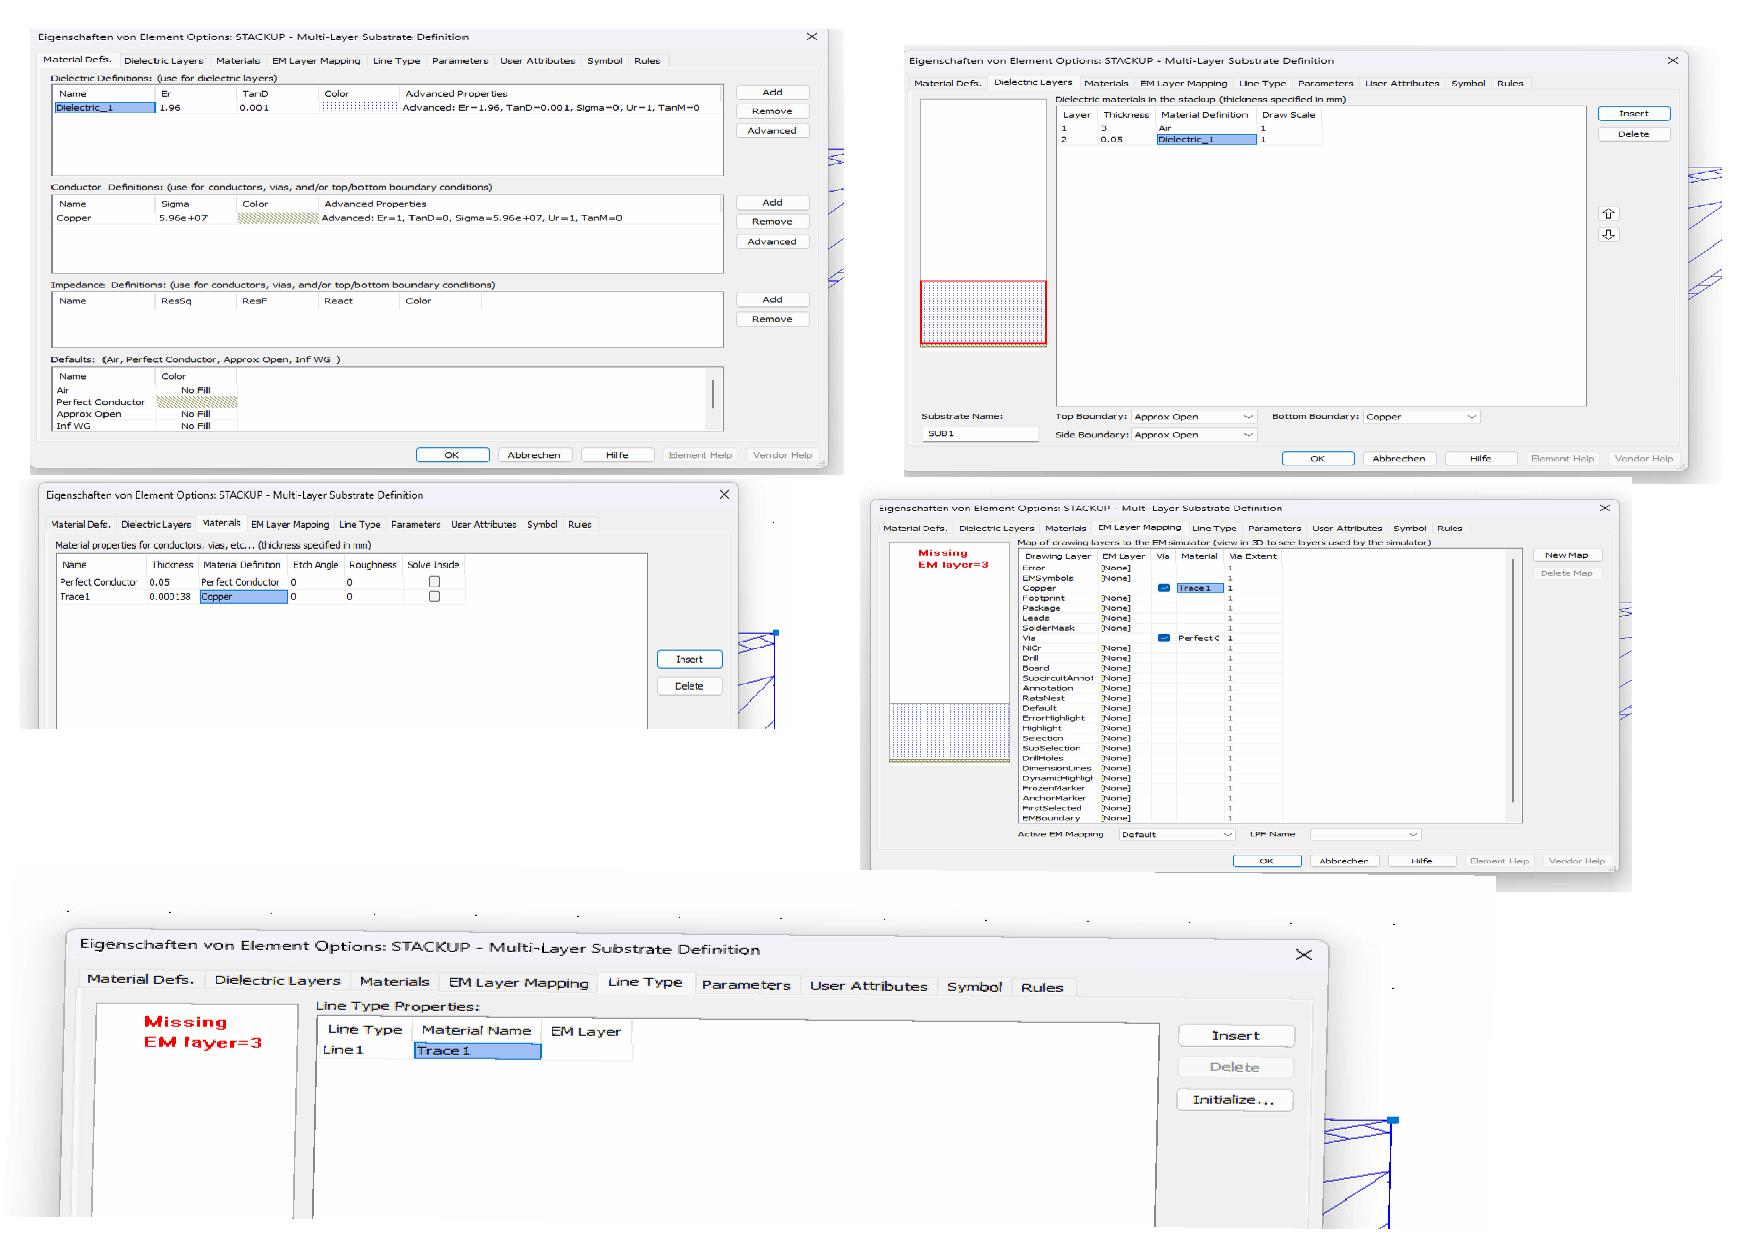
\includegraphics[width=0.8\textwidth]{figures/Em2.pdf}
    \caption{Power measue on AWR schematic and graphs from s parameters}
    \label{Em2}
\end{figure}


then click make new EM structure and chose the simulator as on the \cref{Em3} make new EM structure 
on the EM sturcture check the properties before foolow the video (Basics of setting up and running an EM simulation (AXIEM) in Microwave Office
) to make the setup . then draw rectangle to make a layout, it like drawing the layers of the design. but you have just one layer not many layers as on the pcb.
add ports to the layout  from the icon bedife view 2d layer map icon. 
for the ports make the connect to lower option on the properties. for the two ports, 
the enclosure option slo control the grid size from it. 
the size of the grid controlled from the enclosure tap this also affect the time of simulation fo we need larger size to save the device. memory. 
\begin{figure}[H]
    \centering
    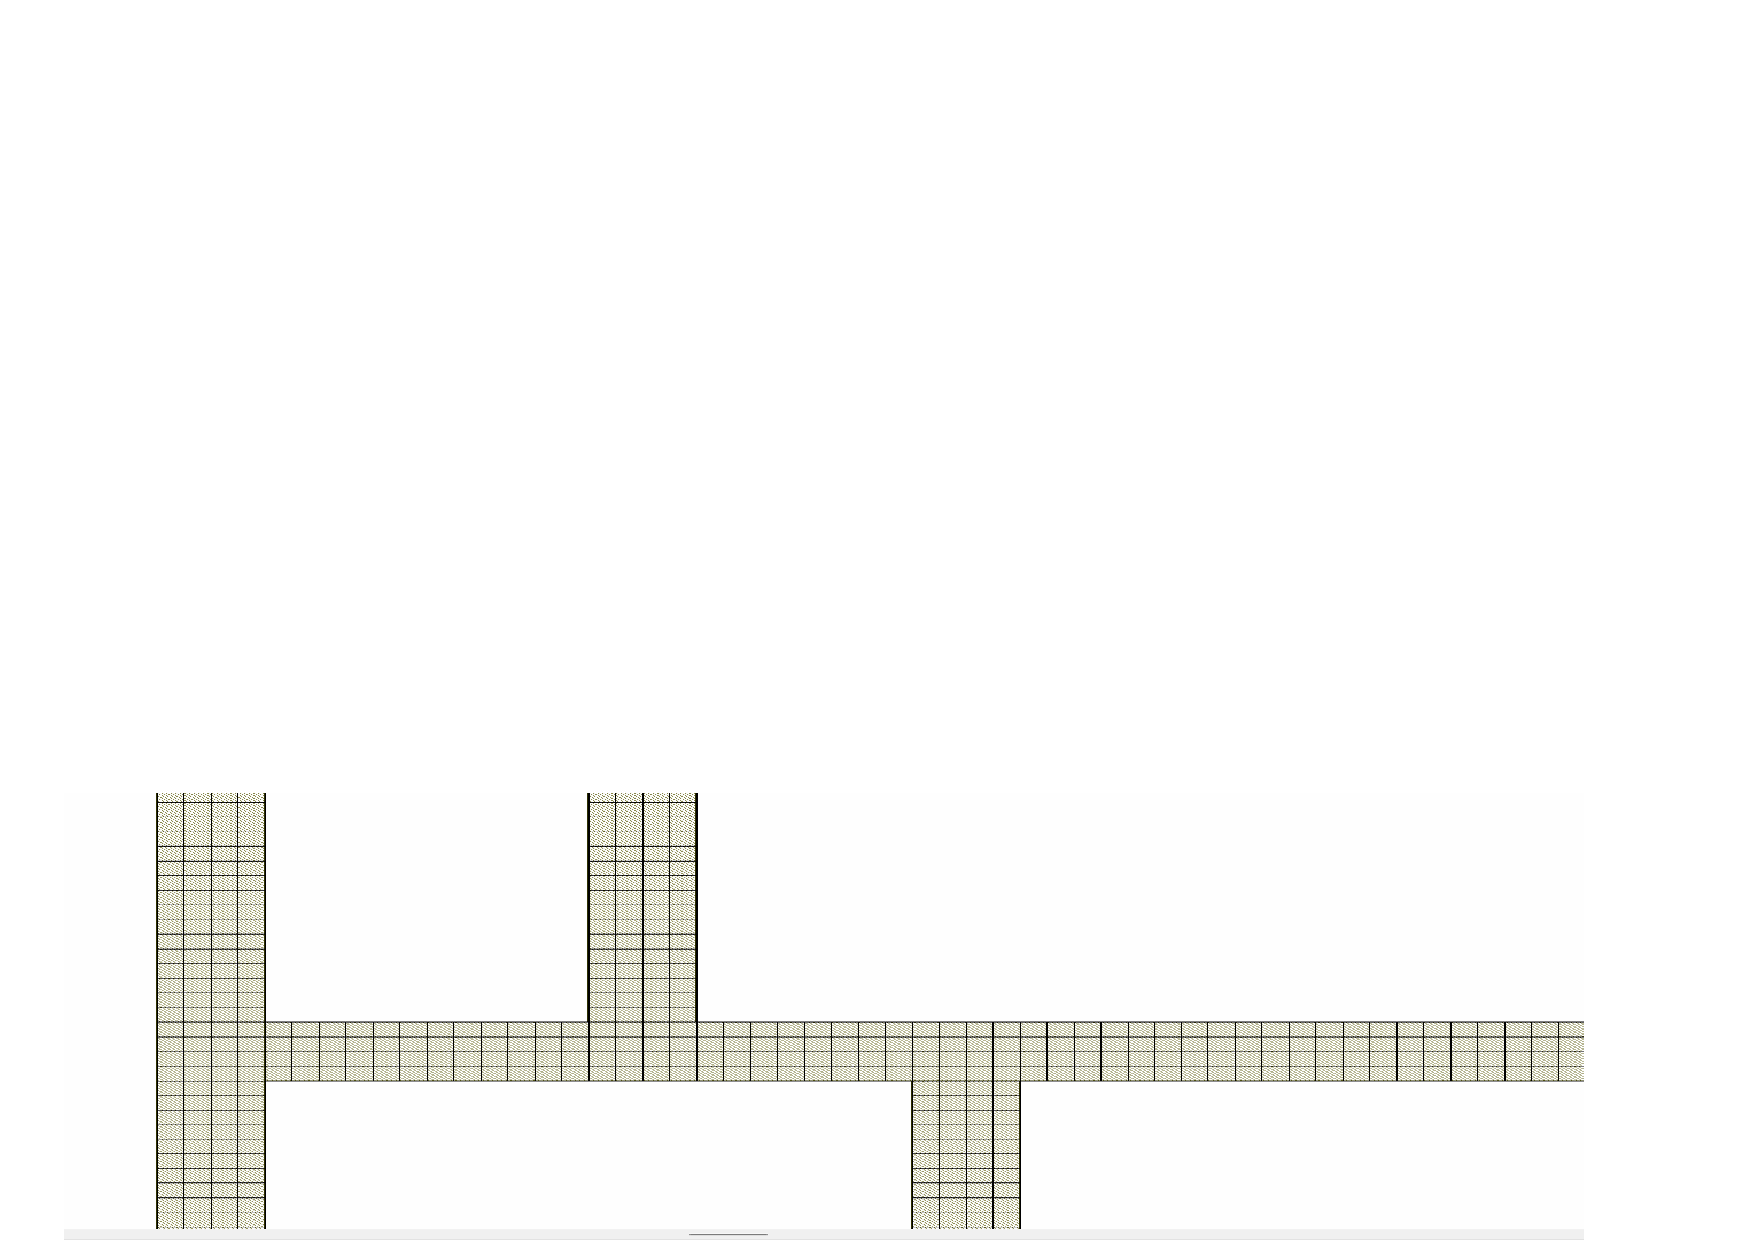
\includegraphics[width=0.8\textwidth]{figures/Em3.pdf}
    \caption{Power measue on AWR schematic and graphs from s parameters}
    \label{Em3}
\end{figure}


from the added ports make the s parameters simulation and mesure db s11 and s21 to make the fileter, 
to check the  current simulation  AFS option as on the figure \cref{Em4} turn it off as it means it will not  simulate every freq we sweep as on the project options.
the current mesurment and it run 3d view is on  te \cref{Em4}  picture my design didn't works as the ports not added correctly to see the simulation follow the video . 
Em sturcture dealing with current is very prictiges and show nice graphs.


\textbf{EM simulation}
\begin{itemize}
    \item aftr you finsh the design and the simulation from scripts- EM - create stackup 
    \item stackup is a multi layer substrate definations based on the substrate we use .it create the substrate definations for EM simulation  
    \item open it properties and any chages on stackup will now  change the design it just will be considered on the EM simulation, 
    \item Etract tool this connect our design to the EM simulation 
    \item AXIEM simulator chosen on the extraction tools, whixh make the design red color when start eM simulation 
    \item the EM simulation is for the layout of the design which is formed from cells the size of the cell controlled for the extraction tool and also it define the number of cells on the design which affect the simulation time. smller cell size more accurate simulation 
    \item  from the element option enable the model option that is used on eM simulation. ths after you sellect  all component you wanna simulate when this model is enabled this mean that the componet are connect with the extraction tool if you click it all the component will be red.
    \item on the extraction tool if right click then add extraction it will show us a design like the layout design 
    \item when the layout open mmake snap together then make add  em extraction it will show nice layout design open the layout and make the matirials coppet this step also can be done from the stackup tools on the matirials option then press add extraction again after you add the a matirials 
    \item the on the layout window press show 2d map it will show the cells of the layout 
    \item if it is very large the simulation time will be very long 
    \item then press simulate and on the graph use the source called design name EM 
    \item then see the difference between EM and normal simulation.
    \item on layout option from options on the upper  toolbar  make snap together sone automatically when make any changes on the circuit as if it is not the extraction model will change if you chages any coomponent parameter.
    \item after any changes on the design update the model from add extraction.
    \item then resimulate the design 
    
\end{itemize}


\textbf{Txline tool}
on the  values chane the dielectric const and the conductor to copper and the dielectric to air and the loss tangent 0.0019 
then on the electrical characteristic change the operating freq and the electrical length. 
on the physical side change the hight based on the datasheet of the microstrip line that you will use. 
also the thickness of the pcb 
on Microwave office add a microstrip to the design and anf the lines you want work with it. 
cand the MSUB values based on the txline calcuation 
to check plot S11 and change the unit to measure the angle not dB and see the point ofthe center freq defined on the txline. 
it should be the same. 



\textbf{Transient analysis}
all the component has the small dash beside it it show the dierction of current this shown on the video for Moffice transient by Aaron Scher.and also the setup and the graphs setup is on the video


\section{Ecplore RF}
\textbf{Basics circuits v1 }


















\textbd{Component tolerence}
\textbf{All the components on the design have a tolerance of  $+ or - \2\%$  more or less }
this will need monto carlo and yiels analysis  there is a video on the Anurag achannel about that after monto carlo simulation you will  see the S11 for example it might be S22 or other  you woll see many values on one  curve  which represent  $ \5\%$ change between the other curve this percent set up during simulation for the design.as \cref{Anurug rf6_3}
then after you get this large number of the measuments make the yield analysis or yield optmization to get the central measument.







































































     










    

\end{itemize}

\textbf{Anurag RF design 9}
\begin{itemize}
    \item some notes about the noise
    \item LNA Theory & Fundamentals - Quick Review

    What is a Low Noise Amplifier?
    
    A low-noise amplifier (LNA) is an electronic amplifier that amplifies a very low-power signal without
    significantly degrading its signal-to-noise ratio.
    An amplifier will increase the ower of both the signal and the noise present at its input, but the amplifier will
    also introduce some additional noise. LNAs are designed to minimize that additional noise.
    V Designers can minimize additional noise by choosing low-noise components, operating points, and
    circuit topologies.
    v Minimizing additional noise must balance with other design goals such as power gain & impedance matching.
    An LNA is a key component at the front-end of a radio
receiver circuit to help reduce unwanted noise in particular. In
most receivers, the overall NF is dominated by the first few
stages of the RF front end.

By using an LNA close to the signal source, the effect of noise from subsequent stages of the receive chain in
the circuit is reduced by the signal gain created by the LNA, while the noise created by the LNA itself is injected
directly into the received signal.


The LNA boosts the desired signals' power while adding as little noise and distortion as possible. The work done
by the LNA enables optimum retrieval of the desired signal in the later stages of the system.
    




    
    \item \begin{figure}[H]
        \centering
        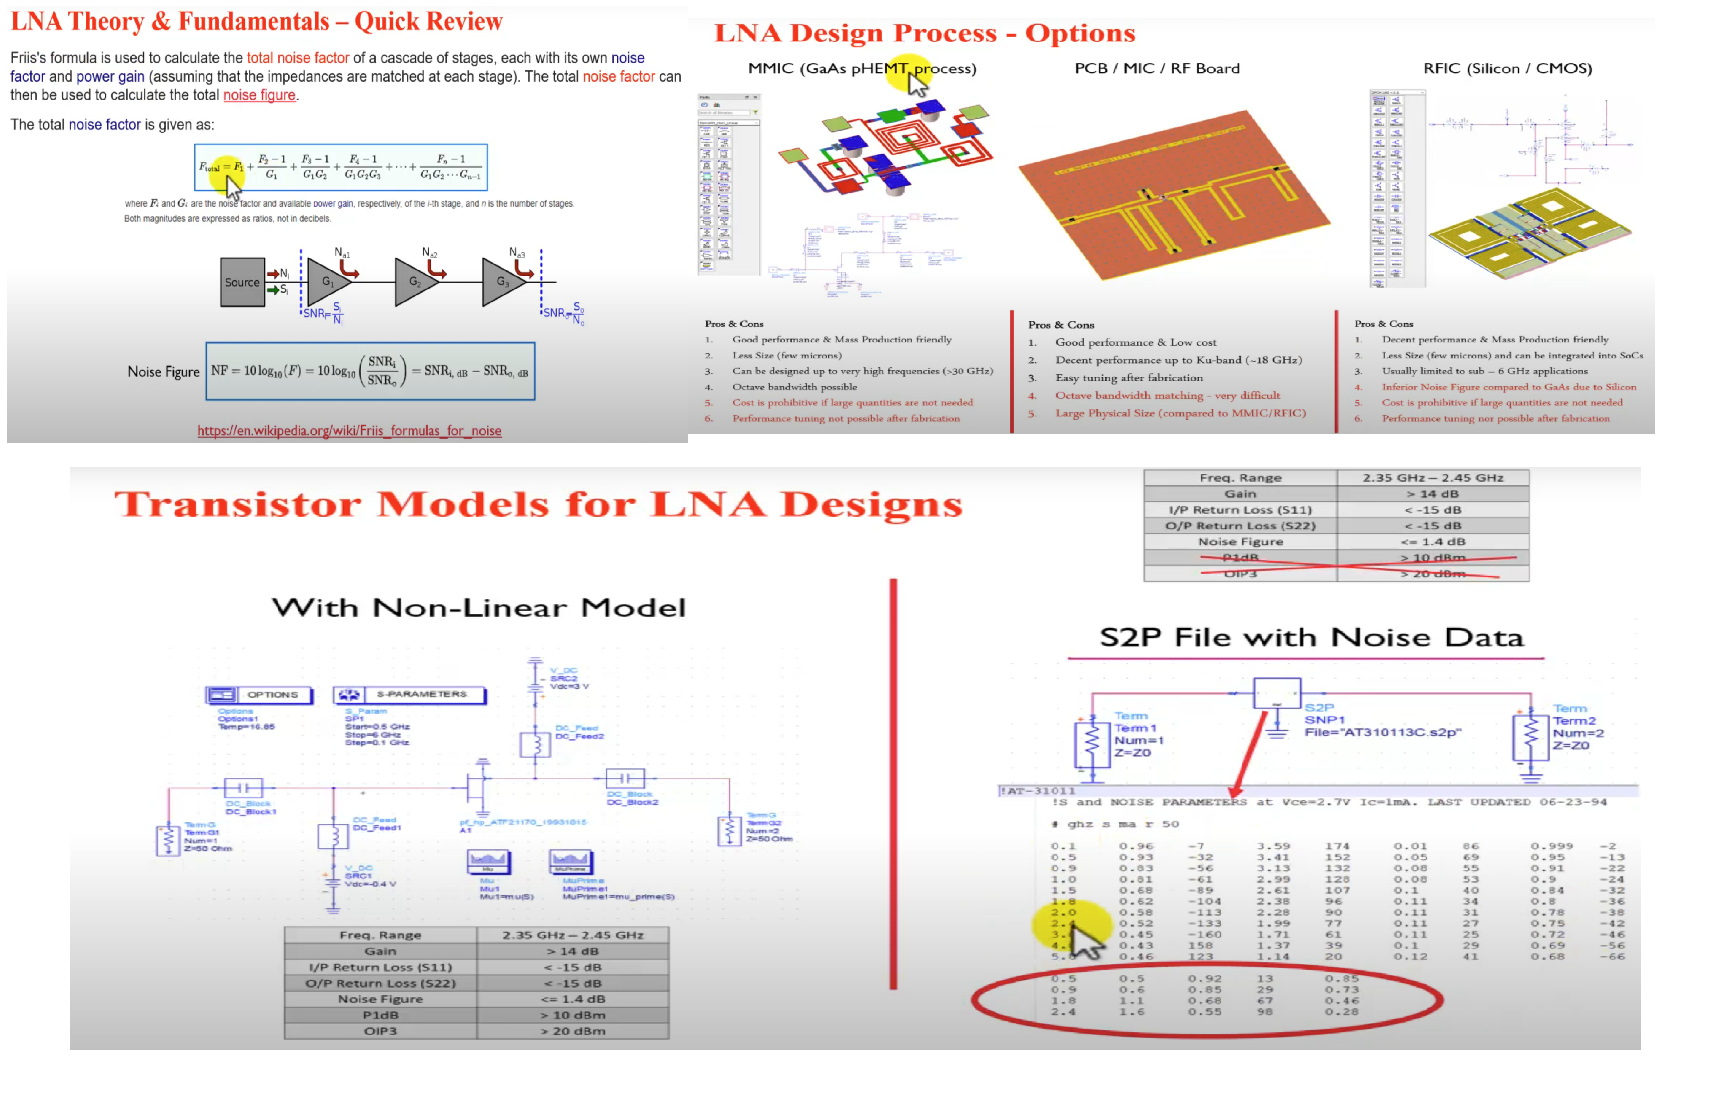
\includegraphics[width=0.8\textwidth]{figures/Noise1.pdf}
        \caption{Stabiliy for transistor and amplifier}
        \label{Noise1}
    \end{figure}
    
\item  if  you are luky you will find the Nonlinear model of your transistor and if not you will have the S2p file that has noise parameter 
at the end of the file and mention the bias point and you will not be able to simulate the Nonlinear points p1dB and oip3 
\item with thr nonlinear model first thinf add biasing for the transistor and get IV curves and check the point you look for it which 
should give as low as possible power consumption which is defined by Vds * Id 
if with s parametr you can't so that as you  have s parameter which is extracted at a  particular bias point .
with s parameter start from the stability point step 2 



\end{itemize}

With the dielectric function $\epsilon$, which describes the response of the material to external electromagnetic fields. $\epsilon = \epsilon_1 + i \epsilon_2$ is a complex function, which will in general depend strongly on the frequency of $\Vec{E}$ and also on the direction, if the material is anisotropic. The sometimes more intuitive complex refractive index $\Tilde{n}$ can be gained from $\epsilon$ throug \cite{paper_2}:

\begin{equation}
    \sqrt{\epsilon} = \Tilde{n} = n + i\kappa
\end{equation}














\subsection{Key Paper 1}
Discuss the first key paper. \cite{author2021paper}

\subsection{Key Paper 2}
Discuss the second key paper. \cite{author2022paper}



\section{Conclusion}
Summarize the key points discussed in the tutorial and their implications.

\bibliographystyle{plain}
\bibliography{references}

\end{document}
